<<<<<<< HEAD
\documentclass[a4paper,10pt,reqno,oneside]{amsart}
\usepackage[footnotesize]{caption}
%\usepackage[usenames,dvipsnames]{color}
%\usepackage[colorlinks=TRUE,linkcolor=Black,urlcolor=Black,citecolor=Black,pagebackref=TRUE,]{hyperref} %Have to change href email.
\usepackage{amsfonts,fancyhdr,graphicx,lastpage,rotating,multirow,fixltx2e, stfloats,txfonts,palatino,url,xcolor,multicol,hanging, setspace,lscape, paralist, changepage,subcaption,array,verbatim,setspace, siunitx,  flafter}
\usepackage[running,displaymath, mathlines]{lineno} % running vs pagewise 
\usepackage{epstopdf}
\renewcommand{\theequation}{eqn \arabic{equation}}
\makeatletter
\def\tagform@#1{\maketag@@@{\ignorespaces#1\unskip\@@italiccorr}}
\makeatother


\usepackage{fancyhdr} 
%\fancyhf{}
\lhead{}
\rhead{}
\chead{Lucas \emph{et al.}: A generalised random encounter model for animals}
\cfoot{\footnotesize{\thepage}}
\pagestyle{fancy}    

\usepackage[nolists, nomarkers, tablesfirst]{endfloat}
\linenumbers
\doublespacing

\usepackage[compress,semicolon]{natbib}

%\renewcommand\thesubfigure{\alph{subfigure}}

% This declares the unit "animals". Also redefined days to be whole word *(not sure if thats what is needed.
\DeclareSIUnit{\animals}{animals}
\DeclareSIUnit{\day}{days}


\captionsetup{width=7cm}


%\usepackage{etoolbox}

\def\r{4}
\def\o{0.3}
\def\lwr{-1.3*\r}
\def\upr{1.3*\r}
\def\gap{0.2}
\def\arrowSz{0.5}
\def\angRad{0.6}
\definecolor{arrowCol}{rgb}{0.5,0.5,0.5}
\definecolor{sensCol}{rgb}{0,0,1}
\definecolor{callCol}{rgb}{1,0,0}

\tikzstyle{profile}=[ultra thick, red]



\newlength{\x}
\newlength{\y}

\newcommand{\call}[1]{ % callAngle
        \fill[opacity=\o, red] (-{\r*sin(#1/2)}, \lwr) rectangle ({\r*sin(#1/2)}, \upr);       
}

\newcommand{\profileOne}[2]{ % sensor width, x1

	\setlength{\x}{#2 pt}
	\setlength{\y}{#1 pt}
	\ifboolexpr{%
		test {\ifdimless{0.5\y}{\x}} 
		and
		test{\ifdimless{\x}{360 pt -0.5\y}} 
	}{
		\pgfmathsetmacro{\leftProf}{max({\r*cos(#2 - #1/2)},{\r*cos(#2 + #1/2)})};
	}{
		\pgfmathsetmacro{\leftProf}{\r};
	}
	\draw[profile]  (0,0)  -- (180:\leftProf)
                        (0,0)  -- (0:\r);  
}



\newcommand{\sensorOne}[2]{ % sensorAngle, x1
	\setlength{\x}{#2 pt}
	\setlength{\y}{#1 pt}
	\ifboolexpr{%
		test {\ifdimless{0.5\y}{\x}} 
		and
		test{\ifdimless{\x}{360 pt -0.5\y}} 
	}{
		\pgfmathsetmacro{\leftProf}{max({\r*cos(#2 - #1/2)},{\r*cos(#2 + #1/2)})};
	}{
		\pgfmathsetmacro{\leftProf}{\r};
	}
        \fill[opacity=\o, blue] (-\leftProf, \lwr) rectangle ({\r}, \upr);       
}

\newcommand{\segmentOne}[2]{ % sensor width, x1
	\draw[] (0,0) -- ++(180 + #1/2 - #2:\r)
     	        (0,0) -- ++(180 - #1/2 - #2:\r);
	\draw[] (0,0) ++(180 + #1/2 - #2:\r) arc (180 + #1/2 - #2:180 - #1/2 - #2:\r);
}

\newcommand{\directionArrowOne}[3]{ % callAngle, sensorAngle, x1
	\setlength{\x}{#3 pt}
	\setlength{\y}{#2 pt}
	\ifboolexpr{%
		test {\ifdimless{0.5\y}{\x}} 
		and
		test{\ifdimless{\x}{360 pt - 0.5\y}} 
	}{
		\pgfmathsetmacro{\leftPoi}{max({\r*cos(#3 - #2/2)},{\r*cos(#3 + #2/2)})};
	}{
		\pgfmathsetmacro{\leftPoi}{\r};
	}
        \pgfmathsetmacro{\rightPoi}{max({\r*sin(#1/2)},{\r)})}
        \fill[ arrowCol ] (-\leftPoi, \lwr-\gap) -- (\rightPoi, \lwr-\gap) -- ({(-\leftPoi+\rightPoi)/2},\lwr-\gap - \arrowSz) -- cycle;

}


\newcommand{\profileTwo}[2]{ % sensor width, x2
        \pgfmathsetmacro{\pLen}{{2*\r*sin(#1/2)*sin(#2)}}
        \draw[profile] (0,0)  ++ (#2 - #1/2:\r) -- ++(180:\pLen) ;
	\draw[profile] (0,0) ++(#2 + #1/2:\r) ++ (0,-\angRad) arc (-90:-(90 - #2):\angRad);
        \node[above right] at (#2 + #1/2:\r) {$x_2$}
}

\newcommand{\sensorTwo}[2]{ % sensorAngle, x2
        \fill[opacity=\o, blue] ({\r*cos(#1/2 + #2)}, \lwr) rectangle ({\r*cos(#2 - #1/2)}, \upr);       
}

\newcommand{\segmentTwo}[2]{ % sensor width, x2
	\draw[] (0,0) -- ++(#2 - #1/2:\r)
     	        (0,0) -- ++(#2 + #1/2:\r);
	\draw[] (0,0) ++(#2 - #1/2:\r) arc (#2 - #1/2:#2 + #1/2:\r);
	\draw[] (0,0) ++(#2 - #1/2:\r) -- (#2 + #1/2:\r);
}

\newcommand{\directionArrowTwo}[3]{ % callAngle, sensorAngle, x2
        \pgfmathsetmacro{\leftPoi}{min({-\r*sin(#1/2)},{\r*cos(#2/2 + #3)})}
        \pgfmathsetmacro{\rightPoi}{max({\r*sin(#1/2)},{\r*cos(#3 - #2/2)})}
        \fill[ arrowCol ] (\leftPoi, \lwr-\gap) -- (\rightPoi, \lwr-\gap) -- ({(\leftPoi+\rightPoi)/2},\lwr-\gap - \arrowSz) -- cycle;

}

\newcommand{\profileThree}[2]{ % sensorAngle, x3
        \pgfmathsetmacro{\pLen}{{\r*sin(#2)}}
        \draw[profile] (0,0) ++ (90 - #2:\r) -- ++(180:\pLen) ;
	\draw[profile] (0,0) ++  (0,\angRad) arc (90:90 - #2:\angRad);
        \node[below right] at (0,0) {$x_3$}
}

\newcommand{\sensorThree}[2]{ % sensorAngle, x3
        \fill[opacity=\o, blue] (0, \lwr) rectangle ({\r*sin(#2)}, \upr);       
}

\newcommand{\segmentThree}[2]{ % sensorAngle, x3
	\draw[] (0,0) -- ++(90 - #2 + #1:\r)
     	        (0,0) -- ++(90 - #2:\r);
	\draw[] (0,0) ++(90 - #2 + #1:\r) arc (90 - #2 + #1:90 - #2:\r);
	\draw[] (0,0) ++(90 - #2 + #1:\r) -- (90 - #2:\r);
}


\newcommand{\directionArrowThree}[3]{ % callAngle, sensorAngle, x3
        \pgfmathsetmacro{\leftPoi}{min({-\r*sin(#1/2)},{0})}
        \pgfmathsetmacro{\rightPoi}{max({\r*sin(#1/2)},{\r*sin(#2)})}
        \fill[ arrowCol ] (\leftPoi, \lwr-\gap) -- (\rightPoi, \lwr-\gap) -- ({(\leftPoi+\rightPoi)/2},\lwr-\gap - \arrowSz) -- cycle;

}



\newcommand{\profileFour}[2]{ % sensor width, x4
        \draw[profile] (0,0)  -- ++(0:\r) ;
	\draw[profile] (0,0) ++ (\angRad,0) arc (0:-#2:\angRad);
        \node[above right] at (0,0) {$x_4$}
}

\newcommand{\sensorFour}[2]{ % sensorAngle, x4
        \fill[opacity=\o, blue] (0, \lwr) rectangle ({\r}, \upr);       
}

\newcommand{\segmentFour}[2]{ % sensor width, x4
	\draw[] (0,0) -- ++(#1 - #2:\r)
     	        (0,0) -- ++(-#2:\r);
	\draw[] (0,0) ++(#1 - #2:\r) arc (#1 - #2:-#2:\r);
	\draw[] (0,0) ++(#1 - #2:\r) -- (-#2:\r);
}

\newcommand{\directionArrowFour}[3]{ % callAngle, sensorAngle, x4
        \pgfmathsetmacro{\leftPoi}{min({-\r*sin(#1/2)},0)}
        \pgfmathsetmacro{\rightPoi}{max({\r*sin(#1/2)},{\r)})}
        \fill[ arrowCol ] (\leftPoi, \lwr-\gap) -- (\rightPoi, \lwr-\gap) -- ({(\leftPoi+\rightPoi)/2},\lwr-\gap - \arrowSz) -- cycle;

}





\newcommand{\fullOne}[3]{ % call, sensor, x4
        \call{#1};
        \sensorOne{#2}{#3};
        \directionArrowOne{#1}{#2}{#3};
        \segmentOne{#2}{#3};
        \profileOne{#2}{#3};
}



\newcommand{\fullTwo}[3]{ % call, sensor, x2
        \call{#1};
        \sensorTwo{#2}{#3};
        \directionArrowTwo{#1}{#2}{#3};
        \segmentTwo{#2}{#3};
        \profileTwo{#2}{#3};
}

\newcommand{\fullThree}[3]{ % call, sensor, x3
        \call{#1};
        \sensorThree{#2}{#3};
        \directionArrowThree{#1}{#2}{#3};
        \segmentThree{#2}{#3};
        \profileThree{#2}{#3};
}



\newcommand{\fullFour}[3]{ % call, sensor, x4
        \call{#1};
        \sensorFour{#2}{#3};
        \directionArrowFour{#1}{#2}{#3};
        \segmentFour{#2}{#3};
        \profileFour{#2}{#3};
}




\begin{document}


\title[Lucas \emph{et al.}: A generalised random encounter model for animals]{A generalised random encounter model for estimating animal density with remote sensor data}
\maketitle

\subsection*{ Running title: A generalised random encounter model for animals}

\subsection*{ Word count:}

\subsection*{ Authors:\\}
Tim C.D. Lucas\textsuperscript{1,2,3}, Elizabeth A. Moorcroft\textsuperscript{1,4,5}, Robin Freeman\textsuperscript{5}, Marcus J. Rowcliffe\textsuperscript{5}, Kate E. Jones\textsuperscript{2,5}


\subsection*{ Addresses:\\}
1 CoMPLEX, University College London, Physics Building, Gower Street, London, WC1E 6BT, UK\\ 
2 Centre for Biodiversity and Environment Research, Department of Genetics, Evolution and Environment, University College London, Gower Street, London, WC1E 6BT, UK\\ 
3 Department of Statistical Science, University College London, Gower Street, London, WC1E 6BT, UK\\ 
4 Department of Computer Science, University College London, Gower Street, London, WC1E 6BT, UK\\ 
5 Institute of Zoology, Zoological Society of London, Regents Park, London, NW1 4RY, UK


\subsection*{ Corresponding authors:\\}
Kate E. Jones,\\
Centre for Biodiversity and Environment Research,\\
Department of Genetics, Evolution and Environment,\\
University College London,\\
Gower Street,\\
London,\\
WC1E 6BT, \\
UK\\
kate.e.jones@ucl.ac.uk\\

Marcus J. Rowcliffe, \\
Institute of Zoology, \\
Zoological Society of London, \\
Regents Park, \\
London, \\
NW1 4RY, \\
UK \\
marcus.rowcliffe@ioz.ac.uk


\clearpage


%max word count 350 words. - current count 347

\section{Abstract}
\subsection*{1:}  Wildlife monitoring technology has advanced rapidly and the use of remote sensors such as camera traps, and acoustic detectors is becoming common in both the terrestrial and marine environments. Current capture-recapture or distance methods to estimate abundance or density require individual recognition of animals or knowing the distance of the animal from the sensor, which is often difficult. A method without these requirements, the random encounter model (REM), has been successfully applied to estimate animal densities from count data generated from camera traps. However, count data from acoustic detectors do not fit the assumptions of the REM due to the directionality of animal signals.

\subsection*{2:} We developed a generalised REM (gREM), to estimate absolute animal density from count data from both camera traps and acoustic detectors. We derived the gREM for different combinations of sensor detection widths and animal signal widths (a measure of directionality). We tested the accuracy and precision of this model using simulations of different combinations of sensor detection widths and animal signal widths, number of captures, and models of animal movement. 

\subsection*{3:} We find that the gREM produces accurate estimates of absolute animal density for all combinations of sensor detection widths and animal signal widths. However, larger sensor detection and animal signal widths were found to be more precise. While the model is accurate for all capture efforts tested, the precision of the estimate increases with the number of captures. We found no effect of different animal movement models tested on the accuracy and precision of the gREM.  

\subsection*{4:} We conclude that the gREM provides an effective method to estimate absolute animal densities from remote sensor count data over a range of sensor and animal signal widths. The gREM is applicable for use for count data obtained in both marine and terrestrial environments, visually or acoustically (e.g., big cats, sharks, birds, bats and cetaceans). As sensors such as camera traps and acoustic detectors become more ubiquitous, the gREM will be increasingly useful for monitoring animal populations across broad spatial, temporal and taxonomic scales. 

\subsection{Keywords} %max keywords/phrase 10 - current 3
Acoustic detection, Camera traps, Marine, Population monitoring, Simulations, Terrestrial 

\section{Introduction}
%Wildlife montoring important (declines in populations, global declines)
%Wildlife monitoring tech growing in sophication and widespread (remote sensors visual and acoustic)
%Difficult to estimate abundance and densities (needed for monitoring)
Animal population density is one of the fundamental measures needed in ecology and conservation. The density of a population has important implications for a range of issues such as sensitivity to stochastic fluctuations \citep{richter1972extinction, wright1983stochastic} and risk of extinction \citep{purvis2000predicting}. Monitoring animal population changes in response to anthropogenic pressure is becoming increasingly important as humans modify habitats and change climates as never before \citep{everatt2014trophic}. % may need more refs 
Sensor technology, such as camera traps \citep{rowcliffe2008surveys, karanth1995estimating} and acoustic detectors \citep{ofarrel1999comparison, clark1995application, acevedo2006using} are becoming increasingly used to monitor changes in animal populations \citep{rowcliffe2008surveys, kessel2014review}, as they are efficient, relativity cheap and non-invasive \citep{cutler1999using}, allowing for surveys over large areas and long periods. However, the problem of converting sampled count data to estimates of density remains as efforts must be made to account for detectability of the animals \citep{anderson2001need}.


%Current methods are often inadequate because of specific data requirements (marked indivudals)
%REM developed for camera trap data, doesnt need this assumptions 
%but has limitations
%Specifically sensor widths - different environments might need more flexibility (examples) and signal directionality assumptions (examples) - method has been optimised for terrestrial large animals
Methods do already exist for estimating animal density if the distance between the animal and the sensor can be estimated (e.g., capture-mark recapture methods \citep{karanth1995estimating} and distance sampling \citep{harris2013applying}). However, these methods often require additional information that may not be available. For example, capture-mark-recapture methods \citep{karanth1995estimating, trolle2003estimation, soisalo2006estimating, trolle2007camera} require recognition of individuals; distance methods require a distance estimation of how far away individuals are from the sensor {barlow2005estimates, marques2011estimating}. The development of the random encounter model (REM) (a modification of a gas model) enabled animal densities to be estimated from unmarked individuals of a known speed, and sensor detection parameters \citep{rowcliffe2008estimating}. The REM method has been successfully applied to estimate animal densities from camera trap surveys \citep{manzo2012estimation, zero2013monitoring}. However, extending the REM method to other types of sensors (for example acoustic detectors) is more problematic, because the original derivation assumes a relatively narrow sensor width (up to $\frac{\pi}{2}$ radians) and that the animal is equally detectable irrespective of its heading (ref). % Find this ref is tricky!

Whilst these restrictions are not problematic for most camera trap makes (e.g. Reconyx, Cuddeback), the REM could not be used to estimate densities from camera traps with a wider sensor width (e.g. canopy monitoring with fish eye lens \citep{brusa2014increasing}). Additionally, the REM method would not be useful in estimating densities from acoustic survey data as the acoustic detector angles are often wider than $\frac{\pi}{2}$ radians.  Acoustic detectors are designed for a range of diverse tasks and environments \citep{kessel2014review}, which will naturally lead to a wide range of sensor detection widths and detection distances. In addition to this, calls emitted by many animals are directional (breaking the assumption of the REM method). 

%acoustic monitoring becoming more common method of monitoring but has additional sensor width problems (examples) and directionality of signals (examples). 
%Currently the count data from acoustic monitoring is used for monitoring in different ways (examples). 
There has been a sharp rise in interest around passive acoustic detectors in recent years, with a 10 fold increase in publications in the decade between 2000 and 2010 \citep{kessel2014review}. Acoustic monitoring is being developed to study many aspects of ecology, including the interactions of animals and their environments \citep{blumstein2011acoustic, rogers2013density}, the presence and relative abundances of species \citep{marcoux2011local}, and biodiversity of an area \citep{depraetere2012monitoring}. 

Acoustic data suffers from many of the problems associated with data from camera trap surveys in that individuals are often unmarked so capture-make-recapture methods cannot be used to estimate densities. In some cases the distance between the animal and the sensor is known, for example when an array of sensors and the position of the animal is estimated by triangulation \citep{lewis2007sperm}. In these situations distance-sampling methods can be applied, a method typically used for marine mammals \citep{rogers2013density}. However, in many cases distance estimation is not possible, for example when single sensors are deployed, a situation typical in the majority of terrestrial acoustic surveys  \citep{elphick2008you, buckland2008estimating}. In these cases, only relative measures of local abundance can be calculated, and not absolute densities. This means that comparison of populations between species and sites is problematic without assuming equal detectability \citep{schmidt2003count}. %Poor reference but the best that I could find
Equality detectability is unlikely because of differences in environmental conditions, sensor type, habitats, species biology. 

In this study we create a generalised REM (gREM), as an extension to the camera trap model of \citep{rowcliffe2008estimating}, to estimate absolute density from count data from acoustic detectors, or camera traps, where the sensor width can vary from 0 to $2\pi$ radians, and the signal given off from the animal can be directional. We assessed the accuracy and precision of the gREM within a simulated environment, by varying the sensor detection widths, animal signal widths, number of captures and models of animal movement. We use the simulation results to recommend best survey practice for estimating animal densities from remote sensors. 

\section{Methods}

\subsection{Analytical Model}

The REM presented by \citep{rowcliffe2008estimating} adapts the gas model to model count data from camera trap surveys. The REM is derived assuming a stationary sensor with a detection width less than $\frac{\pi}{2}$ radians. However, in order to apply this approach more generally, and in particular to acoustic detectors, we need both to relax the constraint on sensor detection width, and allow for animals with directional signals. Consequently, we derive the gREM for any detection width, $ \theta$, between 0 and $2\pi$ with a detection distance $r$ giving a circular sector within which animals can be captured (the detection zone)(Figure~\ref{f:AngleDef}). Additionally, we model the animal as having an associated signal width $\alpha$ between 0 and $2\pi$(Figure~\ref{f:AngleDef}, see Appendix S1 for a list of symbols). We start deriving the gREM with the simplest situation, the gas model where $\theta =  2\pi$ and $ \alpha =  2\pi$. 

%%% Put in new diagram.
\begin{figure}[t]
        \centering
	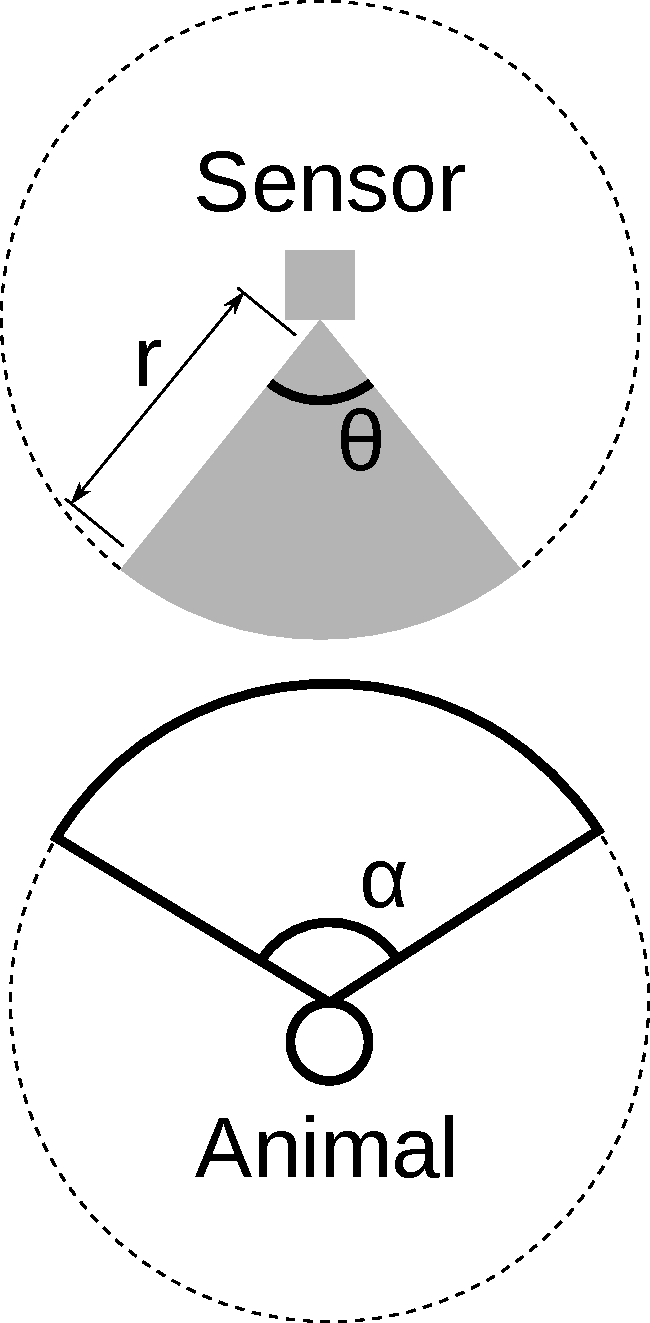
\includegraphics[width=4cm]{imgs/angleDefinitions.pdf}

\caption{Representation of sensor detection width and animal signal width. The filled square and circle represent a sensor and an animal, respectively; $\theta$, sensor detection width (radians); $r$, sensor detection distance; dark grey shaded area, sensor detection zone; $\alpha$, animal signal width (radians). Dashed lines around the filled square and circle represents the maximum extent of $\theta$ and $\alpha$, respectively.} % needs new description for the sensor detection zone  
\label{f:AngleDef}
\end{figure}



\subsubsection{Gas Model}

Following \cite{yapp1956theory}, we derive the gas model where sensors can capture animals in any direction and animal's signal is detectable from any direction($ \theta =  2\pi$ and $ \alpha =  2\pi$). We assume that animals are in a homogeneous environment, and move in straight lines of random direction with velocity $v$. We allow that our stationary sensor can capture animals at a detection distance $r$ and that if an animal moves within this detection zone they are captured with a probability of one, while animals outside the zone are never captured.

In order to derive animal density, we need to consider relative velocity from the reference frame of the animals. Conceptually, this requires us to imagine that all animals are stationary and randomly distributed in space, while the sensor moves with velocity $v$. If we calculate the area covered by the sensor during the survey period we can estimate the number of animals the sensor should capture. As a circle moving across a plane, the area covered by the sensor per unit time is $2rv$. The number of expected captures, $z$, for a survey period of $t$, with an animal density of $D$ is $z = 2rvtD$. To estimate the density, we rearrange to get $D = z/2rvt$.

\subsubsection{gREM derivations for different detection and signal widths}
Different combinations of $\theta$ and $\alpha$ would be expected to occur (e.g., sensors have different detection widths and animals have different signal widths). For different combinations $\theta$ and $\alpha$, the area covered per unit time is no longer given by $2rv$. Instead of the size of the sensor detection zone having a diameter of $2r$, the size changes with the approach angle between the sensor and the animal. For any given signal width and detector width and depending on the angle that the animal approaches the sensor, the width of the area within which an animal can be detected is called the profile, $p$. The size of the profile (averaged across all approach angles) is defined as the average profile $\bar{p}$. However, different combinations of $\theta$ and $\alpha$ need different equations to calcuate $\bar{p}$. 

\begin{figure}
\centering
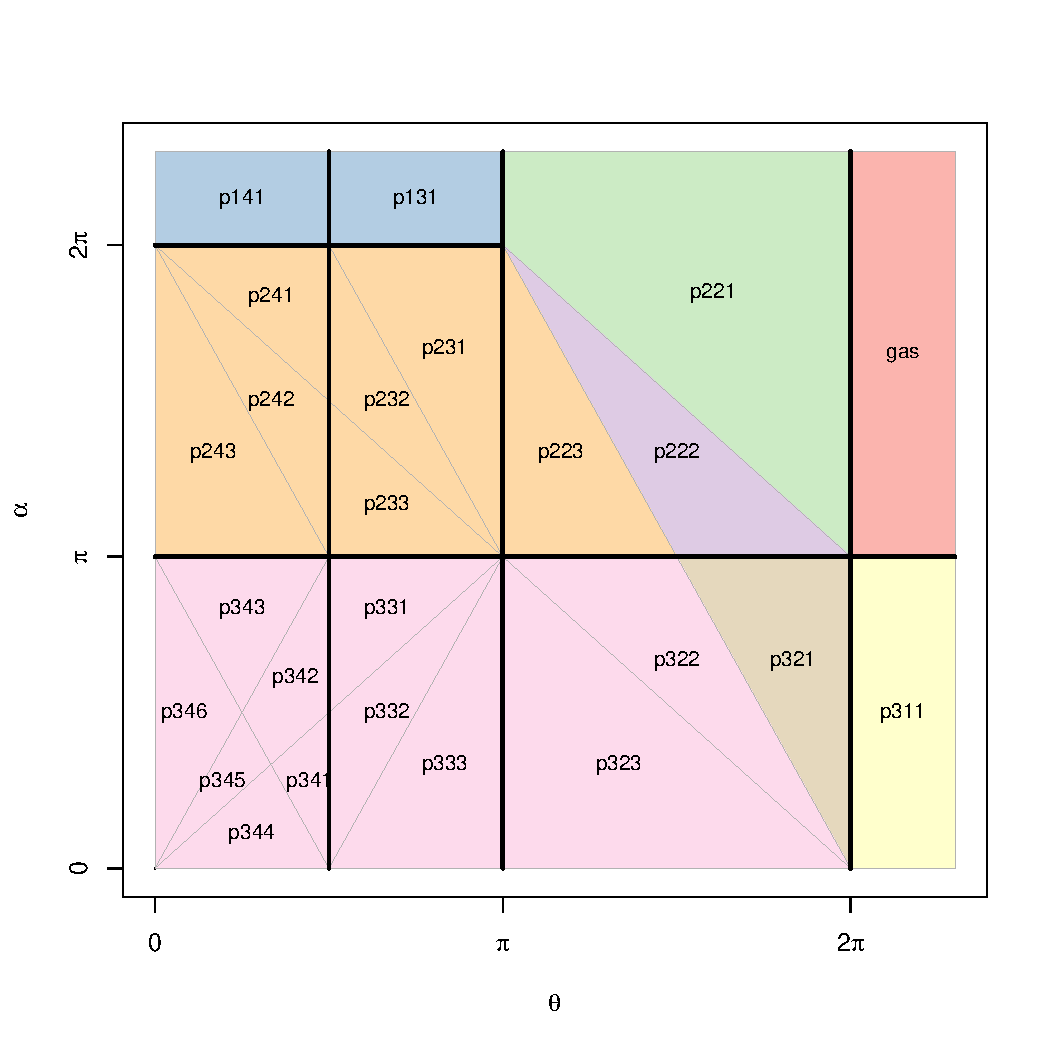
\includegraphics[width=7cm]{imgs/equalRegions.pdf}
\caption{Locations where derivation of the average profile $\bar{p}$ is the same for different combinations of sensor detection width and animal signal width. Symbols within each polygon refer to each gREM submodel named after their compass point, except for Gas and REM which highlight the position of these previously derived models within the gREM.}
\label{f:equalRegions}
\end{figure}

We have identified the parameter space for the combinations of $\theta$ and $\alpha$ for which the derivation of the equations are the same (defined as sub-models in the gREM) (Figure~\ref{f:equalRegions}). For example, the gas model becomes the simplest gREM sub-model (upper right in (Figure~\ref{f:equalRegions}) and the REM from \citep{rowcliffe2008estimating} is another gREM sub-model where $\theta<\frac{\pi}{2}$ and $\alpha = 2\pi$. We derive one gREM sub-model SE2 as an example below (where $4 \pi - 2 \alpha < \theta < 2\pi ,\; 0 < \alpha <\pi$) (see Appendix S2 for other gREM sub-models).

\subsubsection{Example derivation of SE2}

In order to calculate $\bar{p}$, we have to integrate over the focal angle, $x_1$ (Figure~\ref{f:xOne}). This is the angle taken from the centre line of the sensor. Other focal angles are possible ($x_2$, $x_3$, $x_4$) and are used in other gREM sub-models (see Appendix S2). As the size of the profile depends on the approach angle, we present the derivation across all approach angles. When the sensor is directly approaching the animal $x_1  = \frac{\pi}{2}$.

Starting from $x_1 = \frac{\pi}{2}$ until $\frac{\theta}{2} + \frac{\pi}{2} - \frac{\alpha}{2}$, the size of the profile is $2r\sin \frac{\alpha}{2}$ (Figure~\ref{f:firstInt}). During this first interval, the size of $\alpha$ limits the width of the profile. When the animal reaches $x_1$  = $\frac{\theta}{2} + \frac{\pi}{2} - \frac{\alpha}{2}$ (Figure~\ref{f:secondInt}), the size of the profile is $r\sin( \frac{\alpha}{2}) + r\cos( x_1  - \frac{\theta}{2})$ and the size of $\theta/$ and $\alpha$ both limit the width of the profile (Figure~\ref{f:secondInt}). Finally, at $x_1  = \frac{5\pi}{2} - \frac{\theta}{2}  - \frac{\alpha}{2}$ until $x_1  = 3\frac{\pi}{2}$, the width of the profile is again $2r\sin\frac{\alpha}{2}$ (Figure~\ref{f:thirdInt}) and the size of $\alpha$ again limits the width of the profile. 

%insert new figure
\begin{figure}[t]
\captionsetup{width=14cm}
        \centering
	\begin{subfigure}[t]{60mm}
                \centering
		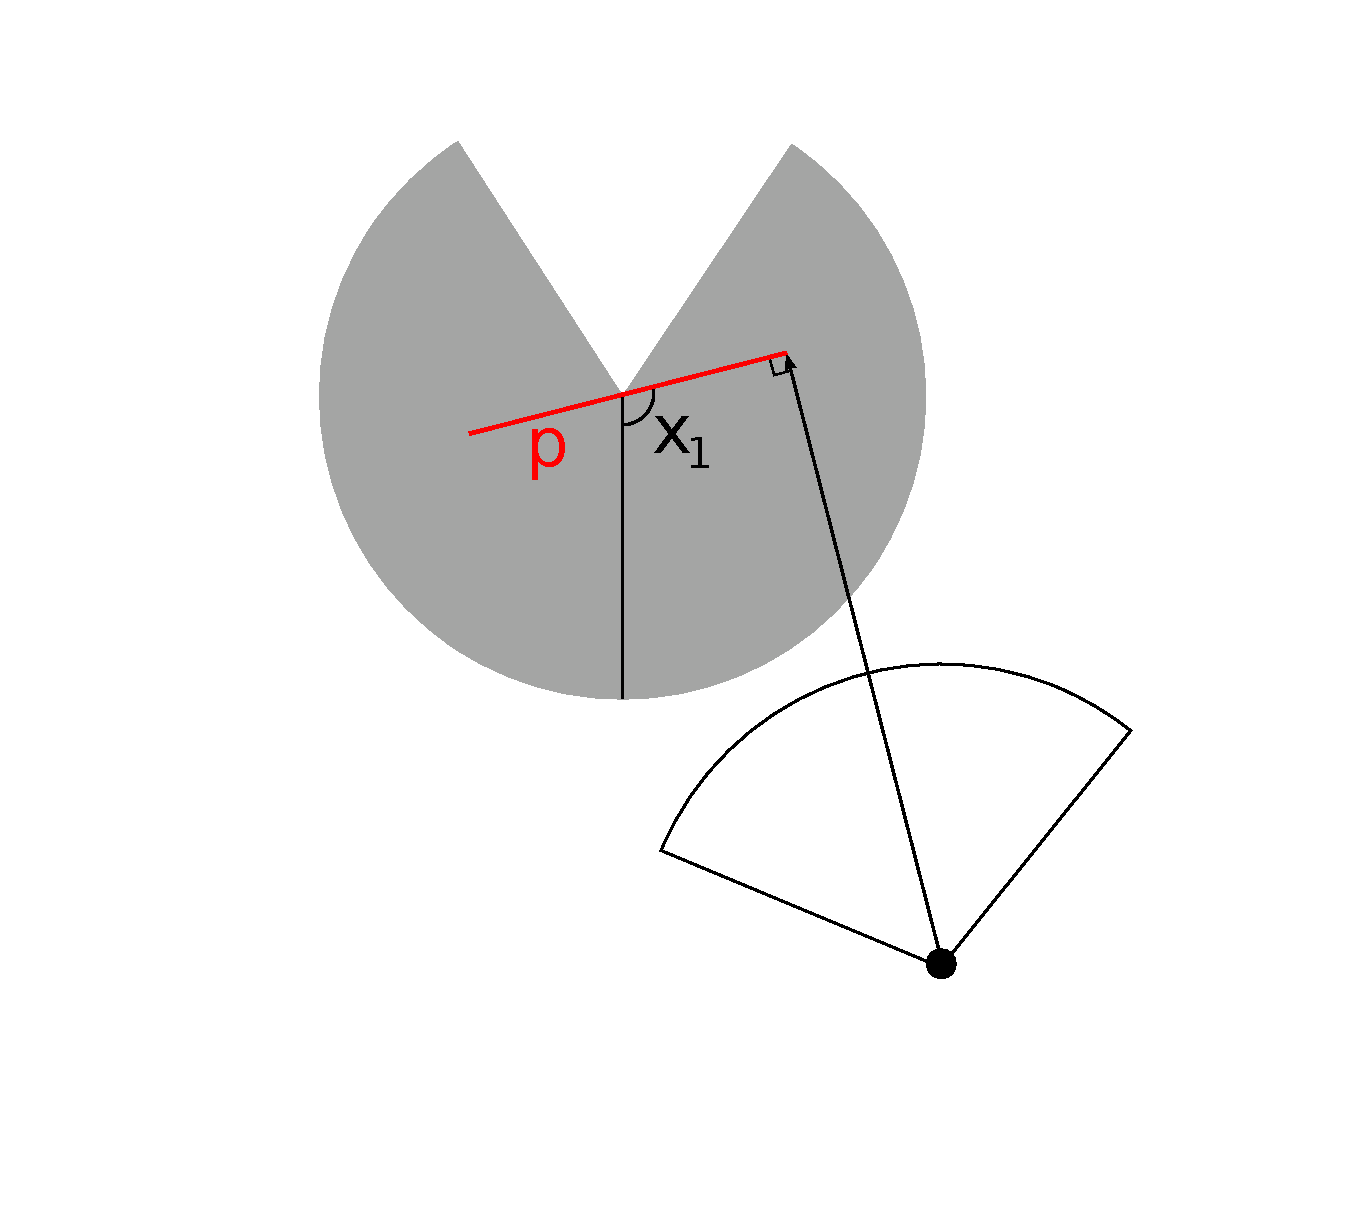
\includegraphics[width=60mm, trim= 6cm 2cm 6cm 0.3cm]{imgs/x1.pdf}
                \caption{}
                \label{f:xOne}
        \end{subfigure}%%
	~ 
	\begin{subfigure}[t]{60mm}
                \centering
		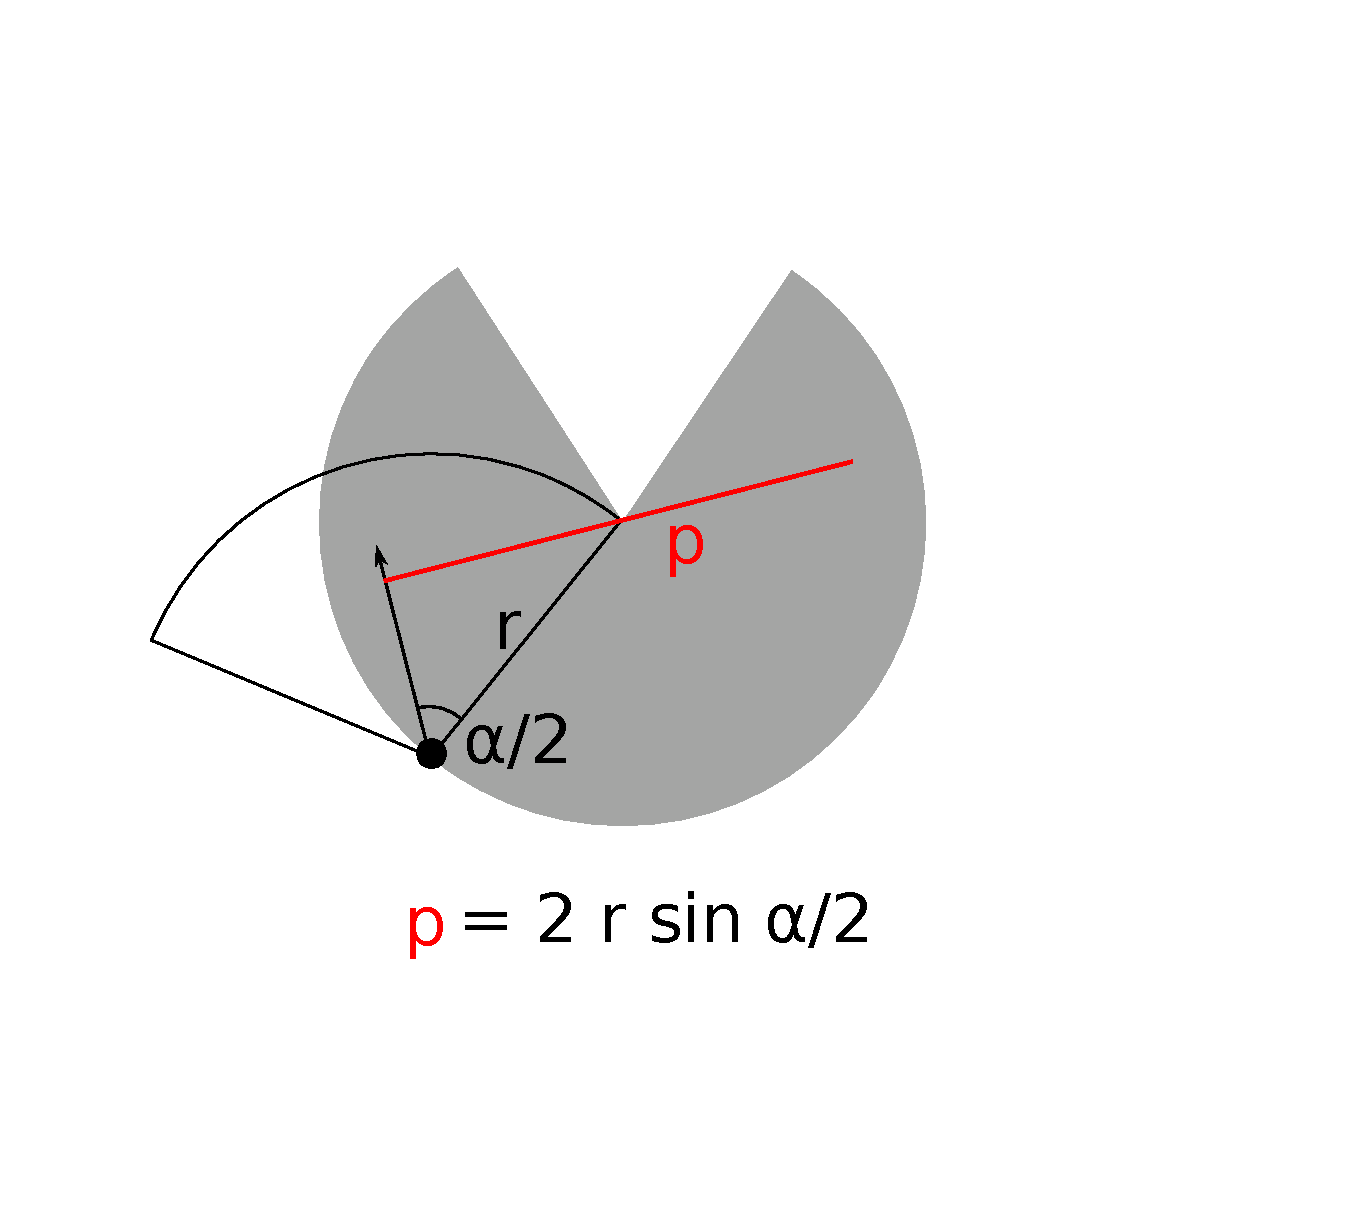
\includegraphics[width=60mm, trim= 6cm 2cm 6cm 4cm]{imgs/firstIntegral.pdf}
                \caption{}
                \label{f:firstInt}
        \end{subfigure}%%
	 
	\begin{subfigure}[t]{60mm}
                \centering
		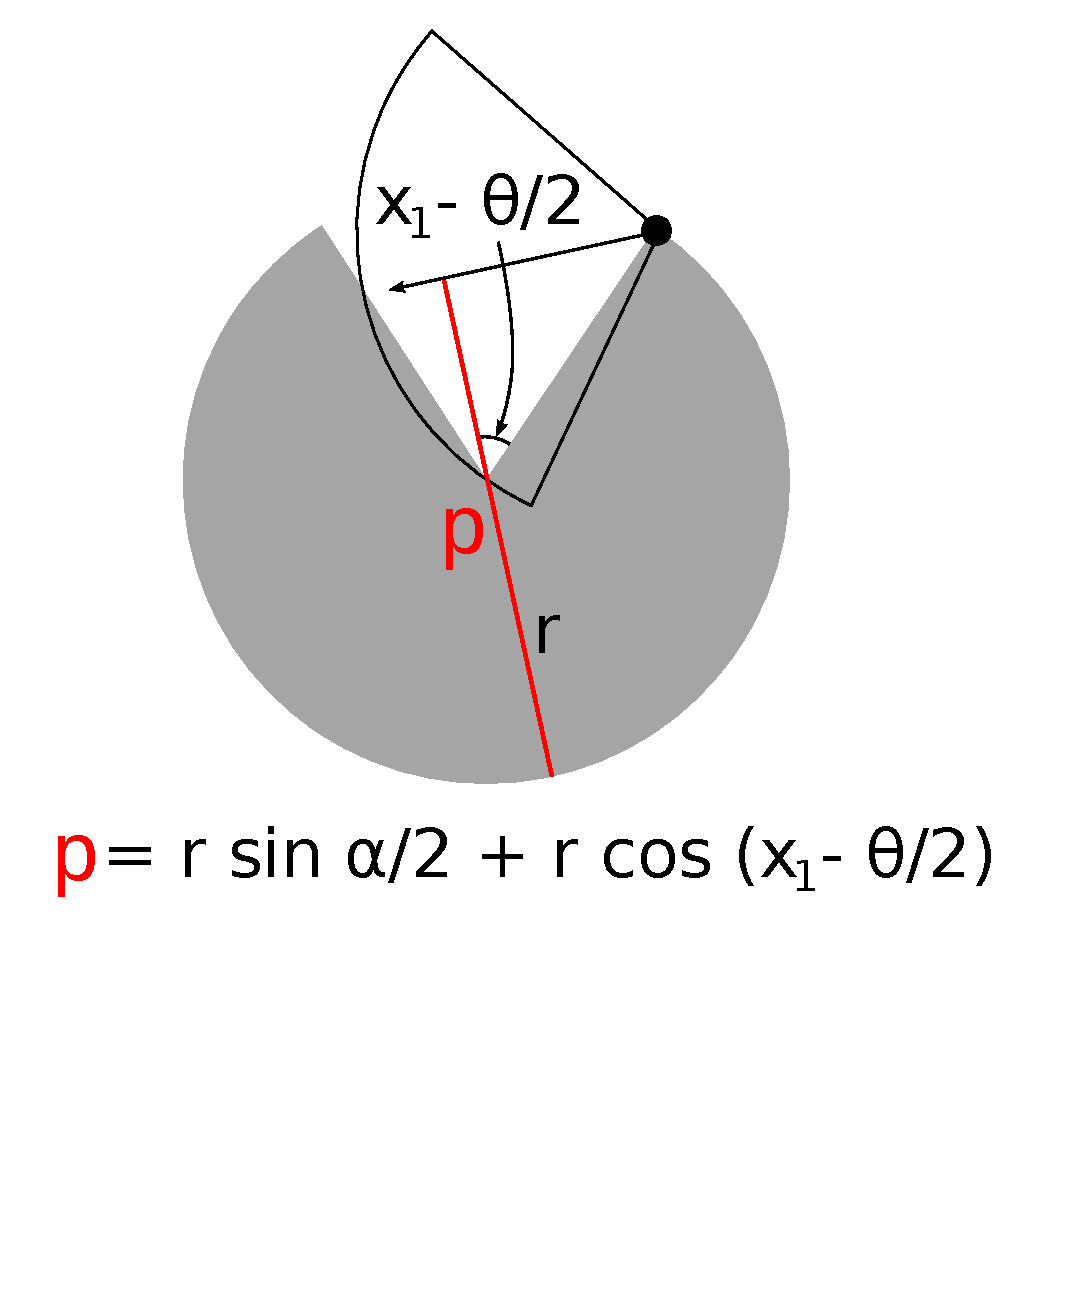
\includegraphics[width=60mm, trim= 6cm 2cm 6cm 1cm]{imgs/secondIntegral.pdf}
                \caption{}
                \label{f:secondInt}
        \end{subfigure}%%
	~ 
	\begin{subfigure}[t]{60mm}
                \centering
		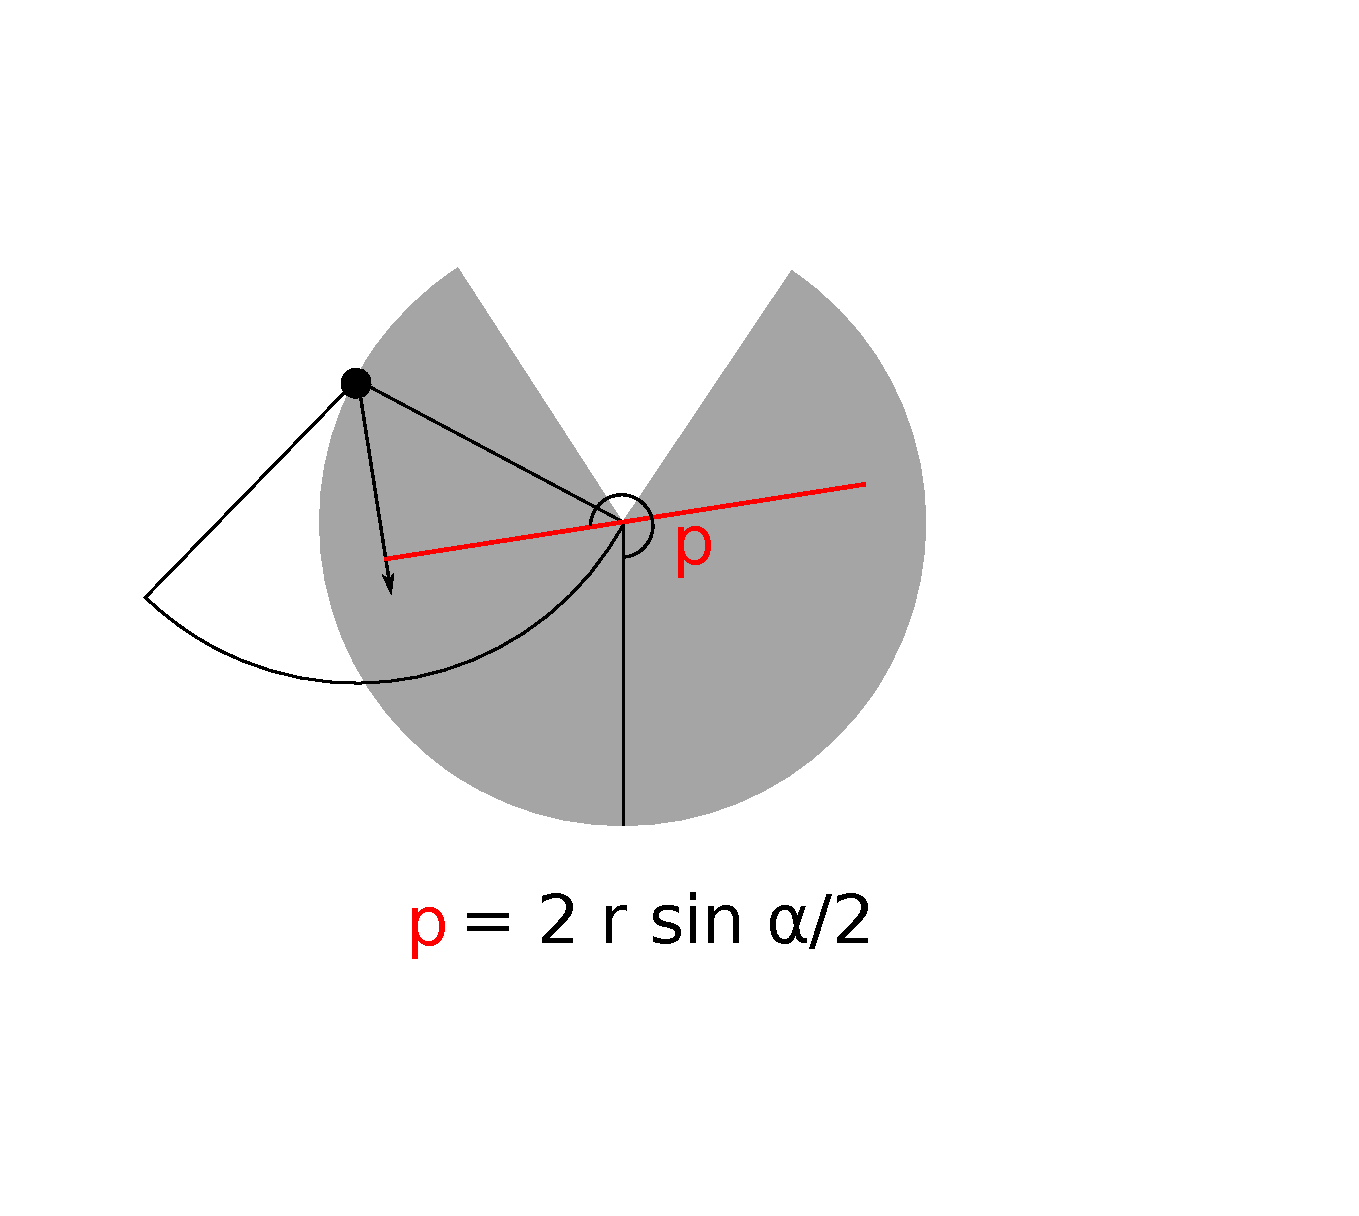
\includegraphics[width=60mm, trim= 6cm 2cm 6cm 4cm]{imgs/thirdIntegral.pdf}
                \caption{}
                \label{f:thirdInt}
        \end{subfigure}%%
\label{f:x1AndInt}
\caption{An overview of the derivation of SE2. The filled circles represent animals, with the animal signal shown as a unfilled sector and the direction of movement shown as an arrow. The detection zone of the sensors are shown as filled grey sectors with a detection distance of $r$. The SYMBOL shows the direction the sensor is facing;  $\theta$, sensor detection width; $\alpha$, animal signal width. The profile $p$ (the line an animal must pass through in order to be captured) is shown in red and $x_1$ is the focal angle, where (a) shows the location of $x_1$. The derivation of $p$ changes as the animal approaches the sensor from different directions where (b) is the derivation of $p$ when $x_1$ is in the interval $\lbrack\frac{\pi}{2}, \frac{\pi}{2} + \frac{\theta}{2} - \frac{\alpha}{2}\rbrack$, (c)  $p$ when $x_1$ is in the interval $\lbrack\frac{\pi}{2} + \frac{\theta}{2} - \frac{\alpha}{2}, \frac{5 \pi}{2} - \frac{\theta}{2} - \frac{\alpha}{2} \rbrack$ and (d) $p$ when $x_1$ is in the interval $\lbrack\frac{5 \pi}{2} - \frac{\theta}{2} - \frac{\alpha}{2}, \frac{3 \pi}{2}\rbrack$. The resultant equation for $p$ is shown beneath each figure.}
\end{figure}

The profile width $p$ for $\pi$ radians of rotation (from directly towards the sensor to directly behind the sensor) is completely characterised by the three intervals (Figure \ref{f:firstInt}--\ref{f:thirdInt}). Average profile width $\bar{p}$ is calculated by integrating these profiles over their appropriate intervals of $x_1$ and dividing by $\pi$ which gives

\begin{align}
    \bar{p} &=\frac{1}{\pi} \left(\int\limits_{\frac{\pi}{2}}^{\frac{\pi}{2} + \frac{\theta}{2} - \frac{\alpha}{2}}2 r \sin{\frac{\alpha}{2} }\;\mathrm{d}x_1+\int\limits_{\frac{\pi}{2} + \frac{\theta}{2} - \frac{\alpha}{2}}^{\frac{5 \pi}{2} - \frac{\theta}{2} - \frac{\alpha}{2}}r \sin{\frac{\alpha}{2} } + r \cos{\left (x_1 - \frac{\theta}{2} \right )}\;\mathrm{d}x_1+\int\limits_{\frac{5 \pi}{2} - \frac{\theta}{2} - \frac{\alpha}{2}}^{\frac{3 \pi}{2}}2 r \sin{\frac{\alpha}{2} }\;\mathrm{d}x_1\right) \nonumber  \\
     &= \frac{r}{\pi} \left(\theta \sin{\frac{\alpha}{2} } - \cos{\frac{\alpha}{2} } + \cos{\left (\frac{\alpha}{2} + \theta \right )}\right). \label{e:p321}
\end{align}

We then, as with the gas model, use this expression to calculate density
\begin{equation}
\label{e:gas}
D = z/vt\bar{p}.
\end{equation}


%fix this @Tim


gREM submodels differ discontinuously (figure 2) at differnt combinations of alpha and theta because the number and nature of intervals needed to describe the average profile width changes.  
Examine the profile at $x_1 = 	\frac{\theta}{2} + \frac{\pi}{2}$ (the profile is perpendicular to the edge of the blind spot.) We see that there is potentially a case where the left side of the profile is $r\sin \frac{\alpha}{2}$ while the right side is zero. This profile does not exist if we return to the full $2r\sin \frac{\alpha}{2}$ profile before $x_1  = \frac{\theta}{2} + \frac{\pi}{2}$. Therefore we solve $\frac{5\pi}{2} - \frac{\theta}{2} - \frac{\alpha}{2} <  \frac{\theta}{2} + \frac{\pi}{2}$. We find that this new profile only exists if $ \alpha < 4\pi - 2 \theta$. This inequality defines the line separating models SE2 and its neighbouring model, SE3.

gREM submodel specifications were done by hand, and the integration was done using SymPy \citep{sympy} in Python (Appendix S3). The gREM submodels were checked by confirming that: 1) submodels adjacent in parameter space were equal at the boundary between them; 2) submodels that border $ \alpha = 0$ had$p = 0$ when $ \alpha = 0$; 3) average profile widths $\bar{p}$ were between 0 and $2r$ and; 4) each integral, divided by the range of angles that it was integrated over, was between 0 and $2r$. The scripts for these tests are included in Appendix S3 and the R \citep{R} implementation of the gREM is given in Appendix S4.  

\subsection{Simulation Model}

We tested the accuracy and precision of the gREM by developing a spatially explicit simulation of the interaction of sensors and animals using different combinations of sensor detection widths, animal signal widths, number of captures, and models of animal movement. 100 simulations were run where each consisted of a  \SI{7.5}{\kilo\meter} by \SI{7.5}{\kilo\meter} square (with periodic boundaries). A stationary sensor of radius $r$ was set up in the exact centre of each simulation, covering 7 sensor detection widths $\theta$ between 0 and $2\pi$(x, x, x, x, x, x). Each simulation was populated with a density of \SI{70}{\animals\per\kilo\meter\squared} to match an expected maximum density of mammals in the wild \citep{damuth1981population}. This created a total of 3937 individuals per simulation which were placed randomly at the start of the simulation. Individuals were assigned x signal detection widths $\alpha$ between 0 and $\pi$ (x,x,x,x,x).

Each simulation lasted for $N$ steps (xx) of duration $T$ (15 minutes) giving a total duration of 150 days. The individuals moved within each step with a distance $d$, with an average speed, $v$. $d$, was sampled from a normal distribution with mean distance, $\mu_d = vT$, and standard deviation $\sigma_d = vT/10$. An average speed, $v = $ \SI{40}{\kilo\meter \per \day}, was chosen as this represents the largest day range of terrestrial animals \citep{carbone2005far}, and represents the upper limit of realistic speeds. At the end step, individuals were allowed to either remain stationary for a time step (with a given propability, $S$), change direction ($A$) between 0 and $\pi$. This resulted in 7 different movement models where: (1) simple movement, where $S$ and $A$ = 0; (2)stop-start movement, where (i) $S$ = 0.25, $A$ = 0, (ii) $S$ = 0.5, $A$ = 0, (iii) $S$ = 0.75, $A$ = 0; (3) random walk movement, where (i) $S$ = 0, $A$ = $\pi/3$, (ii) $S$ = 0, $A$ = $2\pi/3$, iii) $S$ = 0, $A$ = $\pi$.  
Individuals were counted as they moved in and out of the detection zone of the sensor per simulation. 

We calculated the estimated animal density from the gREM by summing the number of captures per simulation and inputting these values into the correct gREM submodel. gREM accuracy was determined by comparing the density in the simulation with the estimated density. High accuracy is indicated by the mean difference between the estimated and actual values converging to zero as sample size increases. gREM precision was determined by the standard deviation of estimated densities. We constructed boxplots of the error between real and estimated densities to graphically test for accuracy and precision. 

We compared the accuracy and precision of all the gREM submodels. As these submodels are derived for different combinations of $\alpha$ and $\theta$, we used the gREM submodel accuracy and precision to determine the impact of different values of $\alpha$ and $\theta$. The impact of the number of captures and animal movement models on accuracy and precision was investigated using 4 different gREM submodels represenative of the range $\alpha$ and $\theta$ values (submodels NW1, SW1, NE1, and SE3, Figure~\ref{f:equalRegions}). Using these four submodels, we calculated how long the simulation needed to run to generate a range of different capture numbers (from 10 to 100 captures in 10 unit intervals), and estimated animal density. These estimated desnities were compared to the real density to assess the impact on the accuracy and precision on the gREM of different simulation lengths. We also used these four submodels to compare the accuracy and precision of a simple movement model, to stop-start movement models and random walk movement models. The gREM assumes that individiuals move continuously with straight-line movement (simple movement model) and we therefore assess the impact of breaking the gREM assumptions. 


\section{Results}

\subsection{Analytical model}

Model results have been derived for each zone with all models except the gas model and REM being newly derived here. However, many models, although derived separately, have the same expression for $p$. Figure~\ref{f:equalModelResults} shows the expression for $p$ in each case. The general equation for density, using the correct expression for $p$ is then substituted into \ref{e:gas}.

Although more thorough checks are performed in Appendix S3, it can be seen that all adjacent expressions in Figure~\ref{f:equalModelResults} are equal when expressions for the boundaries between them are substituted in.

\begin{figure}
\centering
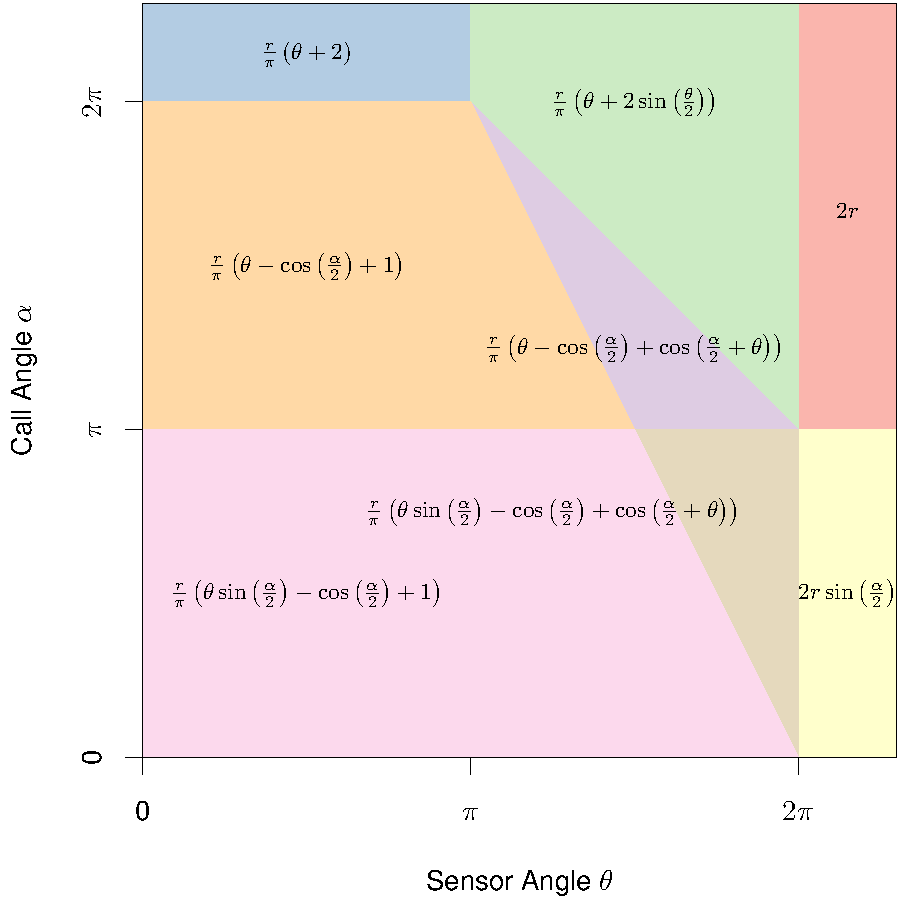
\includegraphics[width=7cm]{imgs/equalModelResults.pdf}
\caption{Equations for the profile wide, $p$, given sensor and call widths. Each colour block represents one equation, despite independent derivation within each block, many models result in the same expression. These are collected together and presented as one block of colour.}
\label{f:equalModelResults}
\end{figure}



\subsection{Simulation model}

\begin{figure}
	\centering
	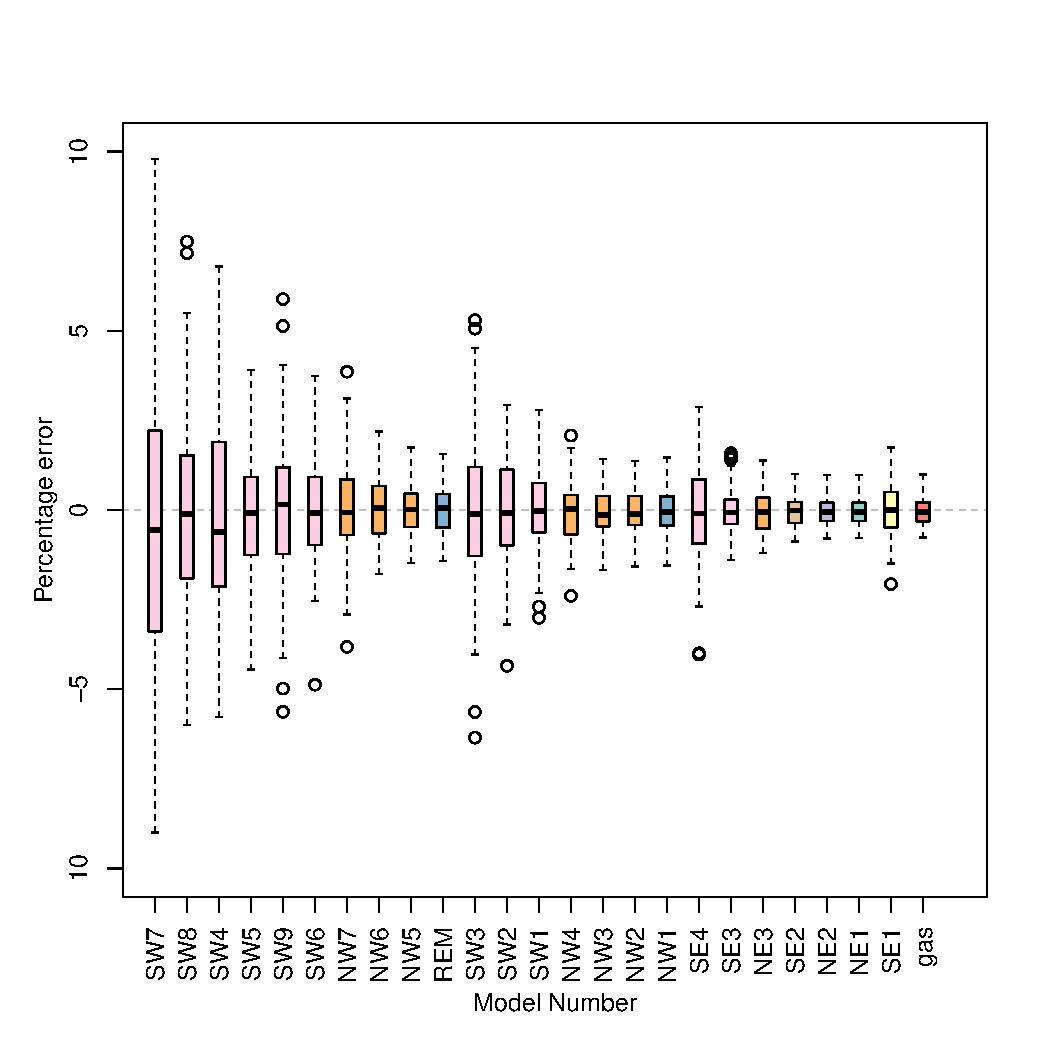
\includegraphics[width=7cm]{imgs/AverageModelBias.pdf}
	\caption{Distribution of the bias for each of the derived models. Percentage error of analytical model calculated from the simulation when settings are: $r = $ \SI{100}{\meter}; $T = $ \SI{150}{\day}; $v = $ \SI{40}{\kilo\meter\per\day}; $D = $ \SI{70}{\animals\per\kilo\meter\squared}; and with detection angles varying between models. The numbers referred to here can be found in Figure 1 Appendix S2, and the colour of each box plot match the functional form of the equation as seen in Figure~\ref{f:equalModelResults}.
  }
	\label{f:ModelBias}
\end{figure}

For each model we compared the estimated densities to the true densities in a simulation. None of the models showed any evidence of any significant differences between the estimated and true density values (Figure~\ref{f:ModelBias}). The precision of the models do vary however. The standard deviation of the error is strongly related to the call and sensor width (Figure~\ref{f:StandardDevaition}), such that larger widths have greater precision. However, even the models with small call and sensor angles have a relativity high level of precision. 

\begin{figure}[t]
        \centering
		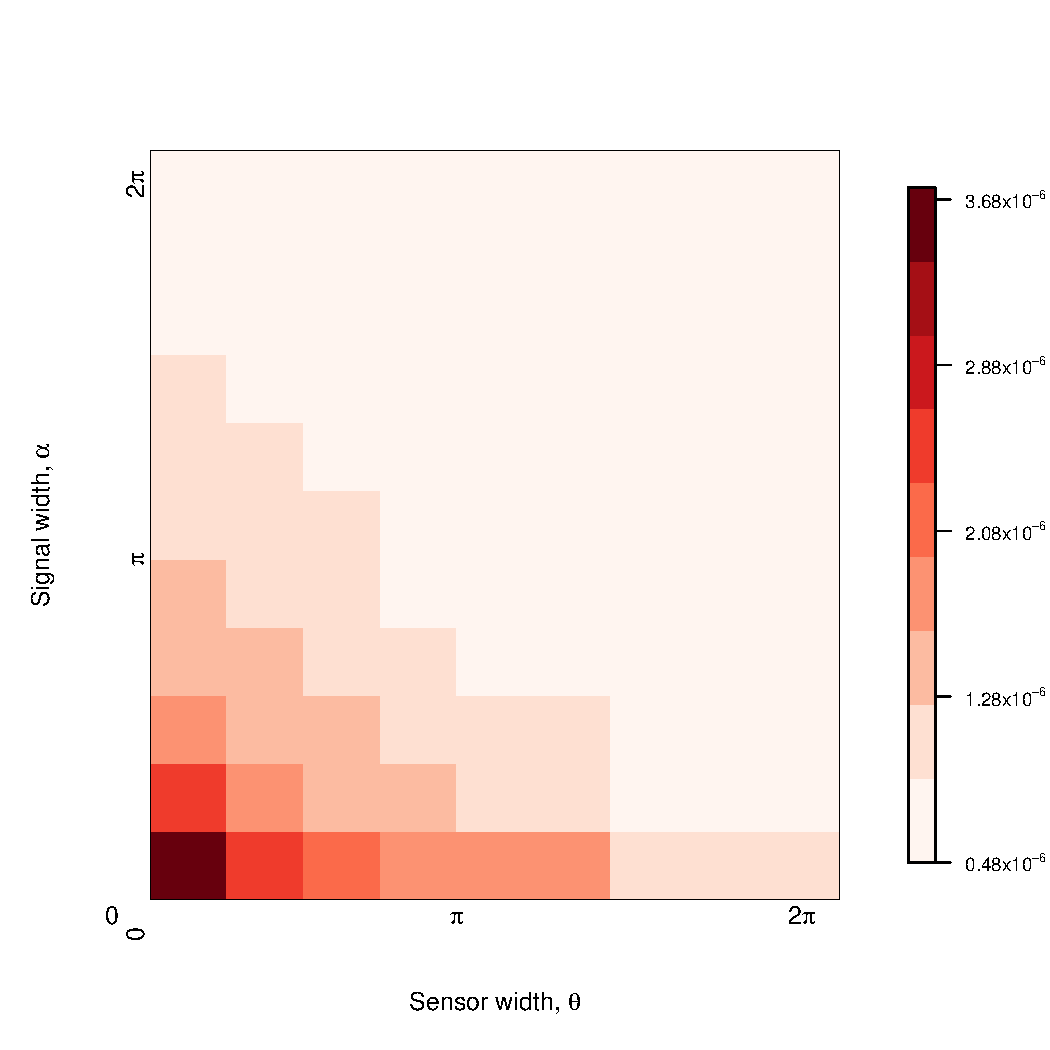
\includegraphics[width=7cm]{imgs/ResultStandardDeviation.pdf}
		%\caption{Angle of detector}
        \caption{The precision of the gREM given a range of detection and call angles. The standard deviation of the percentage error for sensor, and call angles between 0 and $2\pi$ where: $r = $ \SI{100}{\meter}; $T = $ \SI{150}{\day}; $v = $ \SI{40}{\kilo\meter\per\day}; $D = $ \SI{70}{\animals\per\kilo\meter\squared}; and with detection angles varying between models. Where red indicates a high standard deviation and blue represents a low standard deviation.} 
		\label{f:StandardDevaition}
\end{figure}

\begin{figure}[t]
       \centering
	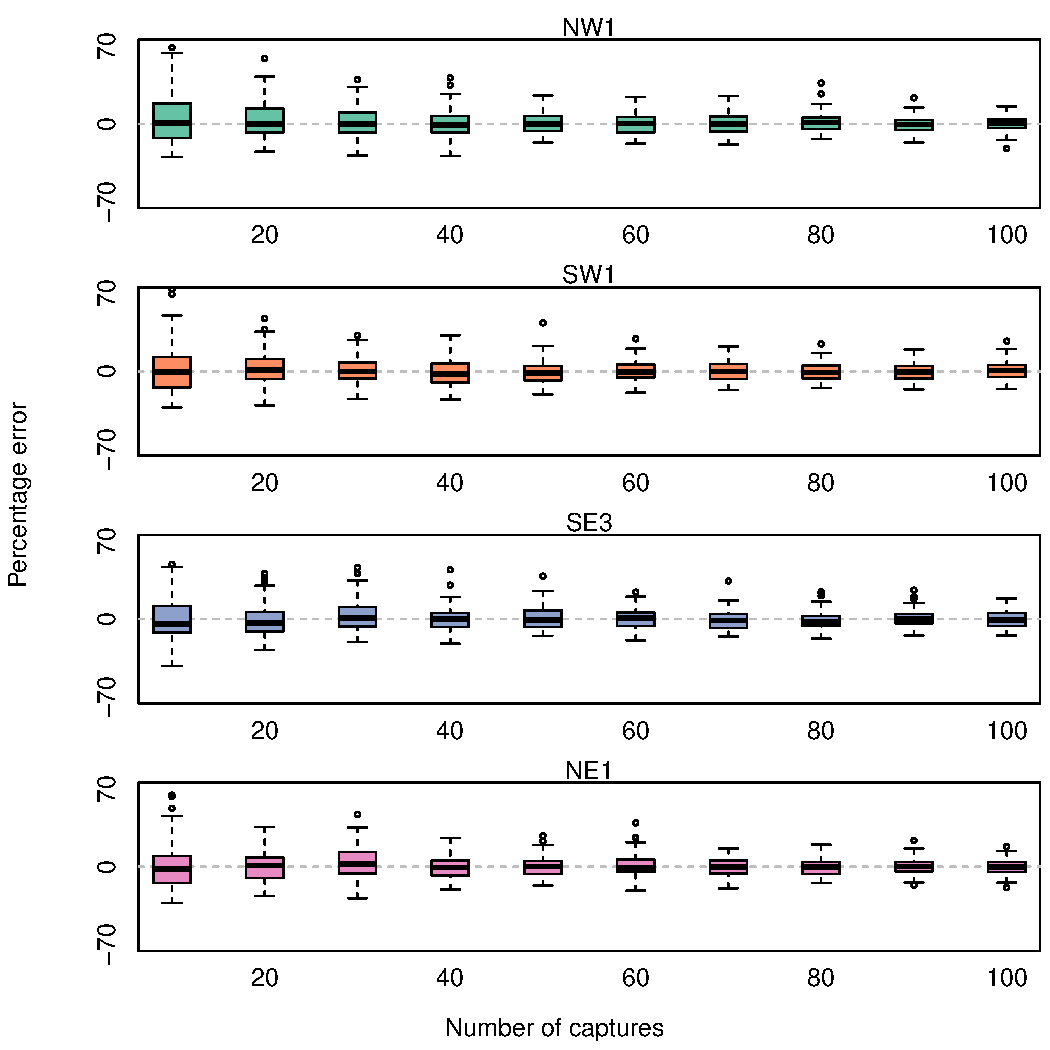
\includegraphics[width=7cm]{imgs/ResultsNoCaptures.pdf}
         %\caption{Number of captures}
           \label{f:Captures}
        \caption{Accuracy of the gREM reminds unchanged, whilst precision increases, with captures. Boxplots of four test models when given different numbers of captures where: $r = $ \SI{100}{\meter}; $T = $ \SI{150}{\day}; $v = $ \SI{40}{\kilo\meter\per\day}; $D = $ \SI{70}{\animals\per\kilo\meter\squared}; and with angles varying between models. Where the model names refer to Figure 1 in Appendix S2.} 
\end{figure}

The precision of the model is dependent on the number of captures during the survey. In Figure~\ref{f:Captures} we can see that the model precision gets greater as the number of captures increase. As the number of captures reaches about 100 then the coefficient of variation falls below 10\% which could be considered negligible. %The number of captures is highly dependent on the speed of the animals, the size of the detection zone, and the length of the survey, as these values increase the number of captures is also likely to increase. 

\subsubsection{Use of the gREM when animal movement is not consistent with model assumptions}

 Simulating start-stop instead of continuous movement had no effect the accuracy, or the precision, of the estimates (Figure~\ref{f:Perch}) as long as the true overall speed of the animal is known. Relaxing straight line movement to allow random or correlated random walks did not effect the accuracy of the method (Figure~\ref{f:Tort}). We allowed animals to change direction up to a maximum value at the end of each step, picked from a uniform distribution where the maximum angle ranged from 0 to $\pi$, which corresponds to straight line movement and random walk respectively. There is no significant difference in the variance for the change, this could be because of the between the step length of the animal movement, 15 minutes, means that immediate double counting of the same animal is unlikely.  In the case where large directional changes are likely to occur within short periods of time leading to double counting of the same animal within a short period of time may need to be adjusted because of this. 

\begin{figure}[t]
      \centering
	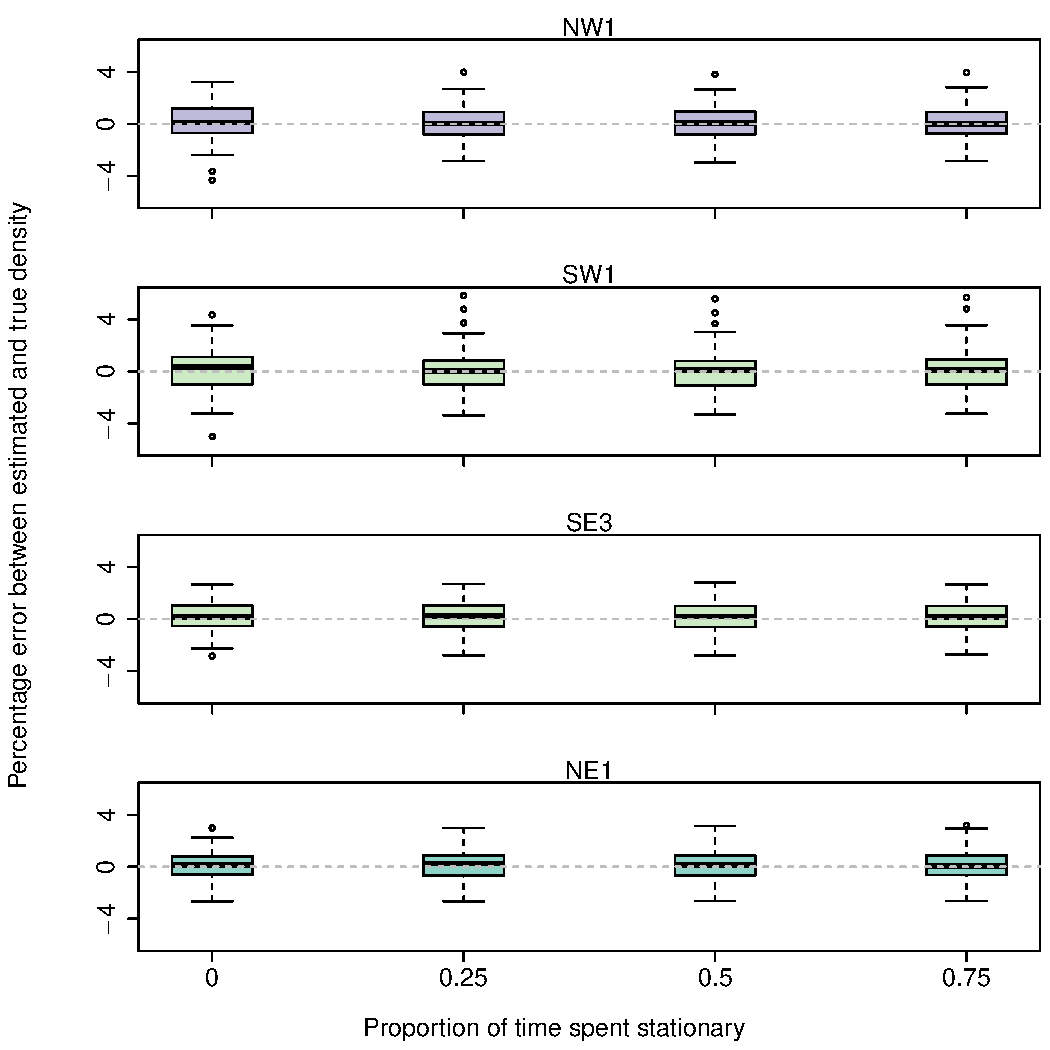
\includegraphics[width=7cm]{imgs/ResultsPerch.pdf}
          %\caption{Proportion of time spent stationary}
          \label{f:Perch}
	\caption{Accuracy and the precision of the gREM given changes in the amount of time an animal spends stationary on average. Distribution of model error when simulated animals spend increasing proportion of time stationary where:  $r = $ \SI{100}{\meter}; $T = $ \SI{150}{\day}; $v = $ \SI{40}{\kilo\meter\per\day}; $D = $ \SI{70}{\animals\per\kilo\meter\squared}; and with detection angles varying between models. Where the model names refer to Figure 1 in Appendix S2. } 
\end{figure}

\begin{figure}[t]
                \centering
		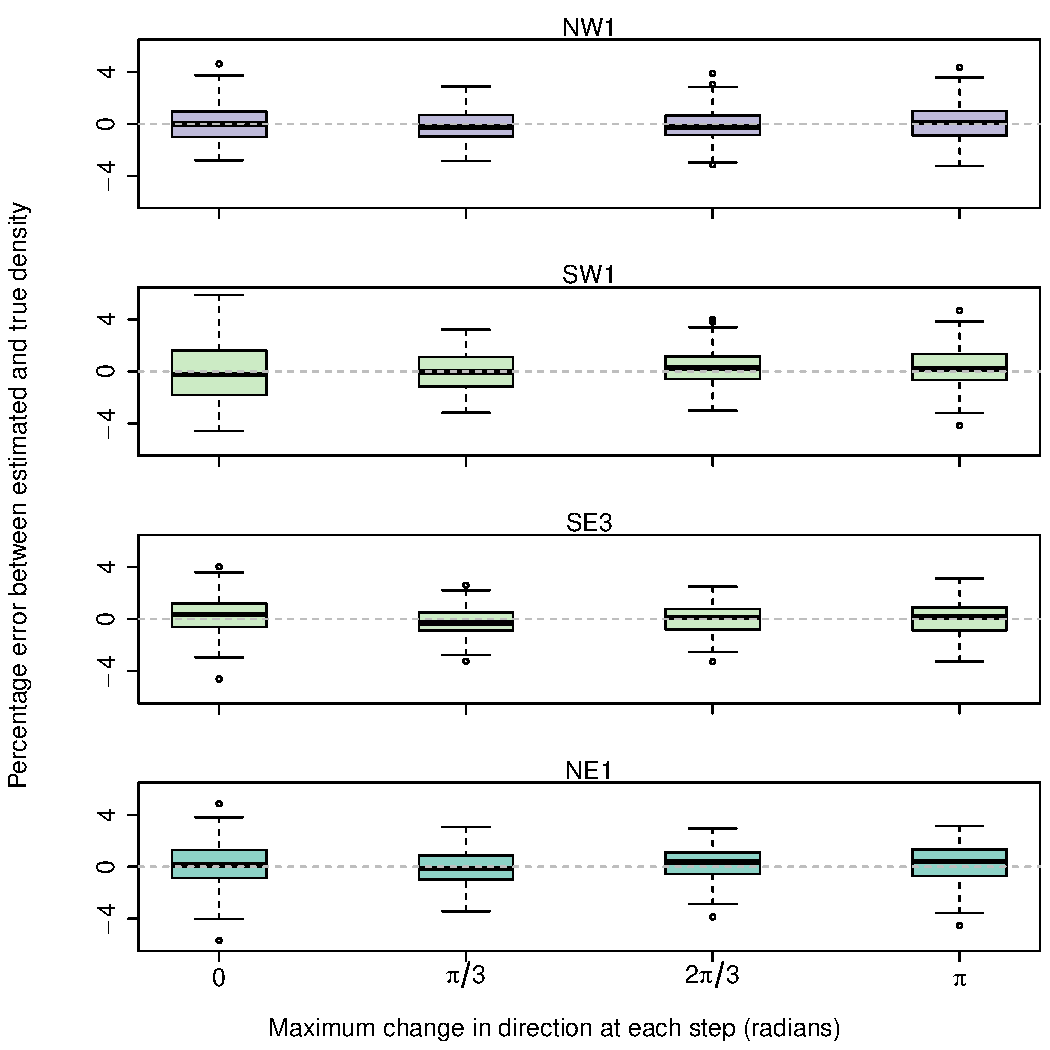
\includegraphics[width=7cm]{imgs/ResultsTort.pdf}
                %\caption{Angle of correlated walk}
                \label{f:Tort}
	\caption{Accuracy and the precision of the gREM given different types of correlated walks. Distribution of model error when simulated animals move with different types of correlated walk where:  $r = $ \SI{10}{\meter}; $T = $ \SI{352}{\day}; $v = $ \SI{40}{\kilo\meter\per\day}; $D = $ \SI{70}{\animals\per\kilo\meter\squared}; and with angles varying between models. Where the model names refer to Figure 1 in Appendix S2.} 
\end{figure}

                  
                  
%%%% ------- Discussion ---------%%%%
\section{Discussion}


We have developed the gREM such that it can be used to estimate density from acoustic and optical sensors. This has entailed a generalisation of the gas model and the model in \citep{rowcliffe2008estimating} to be applicable to any combination of sensor width and call directionality. We have used simulations to show, as a proof of principle, that these models are accurate and precise.

The gREM is therefore available for the estimation of density of a number of taxa of importance to conservation, zoonotic diseases and ecosystem services. The models provided are suitable for certain groups for which there are currently no, or few, effective methods for density estimation. Any species that would be consistently recorded at least once when within range of a detector would be a suitable subject for the gREM, such as bats \citep{kunz2009methods}, songbirds \citep{buckland2006point}, Cetaceans \citep{marques2009estimating} or forest primates \citep{hassel2008reliable}. Within increasing technological capabilities, this list of species is likely to increase dramatically.

Importantly the methods are noninvasive and do not require human marking or naturally identifying marks (as required for mark-recapture models). This makes them suitable for large, continuous monitoring projects with limited human resources. It also makes them suitable for species that are under pressure, species that cannot naturally be individually recognised or species that are difficult or dangerous to catch.

From our simulations  we believe that this method has the potential produce accurate and precise estimates for many different species, using either camera or acoustic detectors. When choosing detectors a researcher should pick the detector with the largest radius and detection angle possible, but whilst a small capture area may reduce precision there is only a limited impact on the overall precision of the model (Figure~\ref{f:StandardDevaition}). A range of factors will affect the overall precision of the model, like size of detection zone, speed of animal, density of animals and length of survey which are reflected in the number of captures. Increasing the number of captures leads to more precise estimates, for species which more slower, or have occur at lower densities, then the detection zone and length of survey need to be increased to compensate so that at least 100 captures are collected (Figure~\ref{f:Captures}).

Within the simulation we have assumed an equal density across the entire world, however in a field environment the situation would be much more complex, with additional variation coming from local changes in density between camera sites. We also assume perfect knowledge of the average speed of an animal and size of the detection zone, and instant triggering of the camera. All of which may lead to possible bias or decreased precision.    

Although we have used simulations to validate these models, much more robust testing is needed. Although difficult, proper field test validation would be required before the models could be fully trusted. Note, however, that the REM \citep{rowcliffe2008estimating} has been field tested. Both \citet{rowcliffe2008estimating} and \citet{zero2013monitoring} both found that the REM were effective manner of estimating animal densities \citep{rowcliffe2008estimating, zero2013monitoring}. There was some discrepancies between the REM and the census methodologies found by Rovero and Marshall which may have been down to lack of knowledge of wild animal speed, and an underestimate in census results \citep{rovero2009camera}. In some taxa gold standard methods of estimating animal density exist, such as capture mark recapture. Where these gold standard exist, and have been proved to work, a simultaneous gREM study could be completed to test the accuracy under field conditions. An easier way to continue to evaluate the models is to run more extensive simulations which break the assumptions of the analytical models. The main element that cannot be analytically treated is the complex movement of real animals. Therefore testing these methods against true animal traces, or more complex movement models would be useful.


There are a number of positive extensions to the gREM which could be developed in the future. The original gas model was formulated for the case where both subjects, either animal and detector, or animal and animal, are moving \citep{Hutchinson_Waser_2007}. Indeed any of the models with animals that are equally detectable in all directions ($\alpha = 2\pi$) can be trivially expanded for moving by substituting the sum of the average animal velocity and the sensor velocity for $v$ as used here. However, when the animal has a directional call, the extension becomes much less simple. The approach would be to calculate again the mean profile width. However, for each angle of approach, one would have to average the profile width for an animal facing in any direction (i.e. not necessarily moving towards the sensor) weighted by the relative velocity of that direction. There are a number of situations where a moving detector and animal could occur and as such may be advantage to have a method of estimating densities from the data collected, e.g. an acoustic detector based off a boat when studying Cetacea or sea birds \citep{yack2013passive}.

Another interesting, and so far unstudied problem, is edge effects caused by trigger delays (the delay between sensing an animal and attempting to record the encounter) and time expansion acoustic detectors which repeatedly turn on an off during sampling. Both of these have potential biases as animals can move through the detection zone without being detected. The models herein are formulated assuming constant surveillance and so the error quickly becomes negligible. For example, if it takes longer for the recording device to be switched on than the length of some animal calls there could be a systematic underestimation of density. 

%%%% ------- Acknowledgments ---------%%%%
\section{Acknowledgments}



\bibliographystyle{mee.bst}	
\bibliography{lucas-moorcroft-etal-refs.bib}	

\end{document}
=======
\documentclass[a4paper,10pt,reqno,oneside]{amsart}
\usepackage[small]{caption}
%\usepackage[usenames,dvipsnames]{color}
%\usepackage[colorlinks=TRUE,linkcolor=Black,urlcolor=Black,citecolor=Black,pagebackref=TRUE,]{hyperref} %Have to change href email.
\usepackage{amsfonts,fancyhdr,graphicx,lastpage,rotating,multirow,fixltx2e, stfloats,txfonts,palatino,url,xcolor,multicol,hanging, setspace,lscape, paralist, changepage,subcaption,array,verbatim,setspace, siunitx,  flafter}
\usepackage[running,displaymath, mathlines]{lineno} % running vs pagewise 
\usepackage{epstopdf}
\renewcommand{\theequation}{eqn \arabic{equation}}
\makeatletter
\def\tagform@#1{\maketag@@@{\ignorespaces#1\unskip\@@italiccorr}}
\makeatother


\usepackage{fancyhdr} 
%\fancyhf{}
\lhead{}
\rhead{}
\chead{Lucas \emph{et al.}: A generalised random encounter model for animals}
\cfoot{\footnotesize{\thepage}}
\pagestyle{fancy}    

\usepackage[nolists, nomarkers, tablesfirst]{endfloat}
\linenumbers
\doublespacing

\usepackage[compress,semicolon]{natbib}

%\renewcommand\thesubfigure{\alph{subfigure}}

% This declares the unit "animals". Also redefined days to be whole word *(not sure if thats what is needed.
\DeclareSIUnit{\animals}{animals}
\DeclareSIUnit{\day}{days}


\captionsetup{width=7cm}


%\usepackage{etoolbox}

\def\r{4}
\def\o{0.3}
\def\lwr{-1.3*\r}
\def\upr{1.3*\r}
\def\gap{0.2}
\def\arrowSz{0.5}
\def\angRad{0.6}
\definecolor{arrowCol}{rgb}{0.5,0.5,0.5}
\definecolor{sensCol}{rgb}{0,0,1}
\definecolor{callCol}{rgb}{1,0,0}

\tikzstyle{profile}=[ultra thick, red]



\newlength{\x}
\newlength{\y}

\newcommand{\call}[1]{ % callAngle
        \fill[opacity=\o, red] (-{\r*sin(#1/2)}, \lwr) rectangle ({\r*sin(#1/2)}, \upr);       
}

\newcommand{\profileOne}[2]{ % sensor width, x1

	\setlength{\x}{#2 pt}
	\setlength{\y}{#1 pt}
	\ifboolexpr{%
		test {\ifdimless{0.5\y}{\x}} 
		and
		test{\ifdimless{\x}{360 pt -0.5\y}} 
	}{
		\pgfmathsetmacro{\leftProf}{max({\r*cos(#2 - #1/2)},{\r*cos(#2 + #1/2)})};
	}{
		\pgfmathsetmacro{\leftProf}{\r};
	}
	\draw[profile]  (0,0)  -- (180:\leftProf)
                        (0,0)  -- (0:\r);  
}



\newcommand{\sensorOne}[2]{ % sensorAngle, x1
	\setlength{\x}{#2 pt}
	\setlength{\y}{#1 pt}
	\ifboolexpr{%
		test {\ifdimless{0.5\y}{\x}} 
		and
		test{\ifdimless{\x}{360 pt -0.5\y}} 
	}{
		\pgfmathsetmacro{\leftProf}{max({\r*cos(#2 - #1/2)},{\r*cos(#2 + #1/2)})};
	}{
		\pgfmathsetmacro{\leftProf}{\r};
	}
        \fill[opacity=\o, blue] (-\leftProf, \lwr) rectangle ({\r}, \upr);       
}

\newcommand{\segmentOne}[2]{ % sensor width, x1
	\draw[] (0,0) -- ++(180 + #1/2 - #2:\r)
     	        (0,0) -- ++(180 - #1/2 - #2:\r);
	\draw[] (0,0) ++(180 + #1/2 - #2:\r) arc (180 + #1/2 - #2:180 - #1/2 - #2:\r);
}

\newcommand{\directionArrowOne}[3]{ % callAngle, sensorAngle, x1
	\setlength{\x}{#3 pt}
	\setlength{\y}{#2 pt}
	\ifboolexpr{%
		test {\ifdimless{0.5\y}{\x}} 
		and
		test{\ifdimless{\x}{360 pt - 0.5\y}} 
	}{
		\pgfmathsetmacro{\leftPoi}{max({\r*cos(#3 - #2/2)},{\r*cos(#3 + #2/2)})};
	}{
		\pgfmathsetmacro{\leftPoi}{\r};
	}
        \pgfmathsetmacro{\rightPoi}{max({\r*sin(#1/2)},{\r)})}
        \fill[ arrowCol ] (-\leftPoi, \lwr-\gap) -- (\rightPoi, \lwr-\gap) -- ({(-\leftPoi+\rightPoi)/2},\lwr-\gap - \arrowSz) -- cycle;

}


\newcommand{\profileTwo}[2]{ % sensor width, x2
        \pgfmathsetmacro{\pLen}{{2*\r*sin(#1/2)*sin(#2)}}
        \draw[profile] (0,0)  ++ (#2 - #1/2:\r) -- ++(180:\pLen) ;
	\draw[profile] (0,0) ++(#2 + #1/2:\r) ++ (0,-\angRad) arc (-90:-(90 - #2):\angRad);
        \node[above right] at (#2 + #1/2:\r) {$x_2$}
}

\newcommand{\sensorTwo}[2]{ % sensorAngle, x2
        \fill[opacity=\o, blue] ({\r*cos(#1/2 + #2)}, \lwr) rectangle ({\r*cos(#2 - #1/2)}, \upr);       
}

\newcommand{\segmentTwo}[2]{ % sensor width, x2
	\draw[] (0,0) -- ++(#2 - #1/2:\r)
     	        (0,0) -- ++(#2 + #1/2:\r);
	\draw[] (0,0) ++(#2 - #1/2:\r) arc (#2 - #1/2:#2 + #1/2:\r);
	\draw[] (0,0) ++(#2 - #1/2:\r) -- (#2 + #1/2:\r);
}

\newcommand{\directionArrowTwo}[3]{ % callAngle, sensorAngle, x2
        \pgfmathsetmacro{\leftPoi}{min({-\r*sin(#1/2)},{\r*cos(#2/2 + #3)})}
        \pgfmathsetmacro{\rightPoi}{max({\r*sin(#1/2)},{\r*cos(#3 - #2/2)})}
        \fill[ arrowCol ] (\leftPoi, \lwr-\gap) -- (\rightPoi, \lwr-\gap) -- ({(\leftPoi+\rightPoi)/2},\lwr-\gap - \arrowSz) -- cycle;

}

\newcommand{\profileThree}[2]{ % sensorAngle, x3
        \pgfmathsetmacro{\pLen}{{\r*sin(#2)}}
        \draw[profile] (0,0) ++ (90 - #2:\r) -- ++(180:\pLen) ;
	\draw[profile] (0,0) ++  (0,\angRad) arc (90:90 - #2:\angRad);
        \node[below right] at (0,0) {$x_3$}
}

\newcommand{\sensorThree}[2]{ % sensorAngle, x3
        \fill[opacity=\o, blue] (0, \lwr) rectangle ({\r*sin(#2)}, \upr);       
}

\newcommand{\segmentThree}[2]{ % sensorAngle, x3
	\draw[] (0,0) -- ++(90 - #2 + #1:\r)
     	        (0,0) -- ++(90 - #2:\r);
	\draw[] (0,0) ++(90 - #2 + #1:\r) arc (90 - #2 + #1:90 - #2:\r);
	\draw[] (0,0) ++(90 - #2 + #1:\r) -- (90 - #2:\r);
}


\newcommand{\directionArrowThree}[3]{ % callAngle, sensorAngle, x3
        \pgfmathsetmacro{\leftPoi}{min({-\r*sin(#1/2)},{0})}
        \pgfmathsetmacro{\rightPoi}{max({\r*sin(#1/2)},{\r*sin(#2)})}
        \fill[ arrowCol ] (\leftPoi, \lwr-\gap) -- (\rightPoi, \lwr-\gap) -- ({(\leftPoi+\rightPoi)/2},\lwr-\gap - \arrowSz) -- cycle;

}



\newcommand{\profileFour}[2]{ % sensor width, x4
        \draw[profile] (0,0)  -- ++(0:\r) ;
	\draw[profile] (0,0) ++ (\angRad,0) arc (0:-#2:\angRad);
        \node[above right] at (0,0) {$x_4$}
}

\newcommand{\sensorFour}[2]{ % sensorAngle, x4
        \fill[opacity=\o, blue] (0, \lwr) rectangle ({\r}, \upr);       
}

\newcommand{\segmentFour}[2]{ % sensor width, x4
	\draw[] (0,0) -- ++(#1 - #2:\r)
     	        (0,0) -- ++(-#2:\r);
	\draw[] (0,0) ++(#1 - #2:\r) arc (#1 - #2:-#2:\r);
	\draw[] (0,0) ++(#1 - #2:\r) -- (-#2:\r);
}

\newcommand{\directionArrowFour}[3]{ % callAngle, sensorAngle, x4
        \pgfmathsetmacro{\leftPoi}{min({-\r*sin(#1/2)},0)}
        \pgfmathsetmacro{\rightPoi}{max({\r*sin(#1/2)},{\r)})}
        \fill[ arrowCol ] (\leftPoi, \lwr-\gap) -- (\rightPoi, \lwr-\gap) -- ({(\leftPoi+\rightPoi)/2},\lwr-\gap - \arrowSz) -- cycle;

}





\newcommand{\fullOne}[3]{ % call, sensor, x4
        \call{#1};
        \sensorOne{#2}{#3};
        \directionArrowOne{#1}{#2}{#3};
        \segmentOne{#2}{#3};
        \profileOne{#2}{#3};
}



\newcommand{\fullTwo}[3]{ % call, sensor, x2
        \call{#1};
        \sensorTwo{#2}{#3};
        \directionArrowTwo{#1}{#2}{#3};
        \segmentTwo{#2}{#3};
        \profileTwo{#2}{#3};
}

\newcommand{\fullThree}[3]{ % call, sensor, x3
        \call{#1};
        \sensorThree{#2}{#3};
        \directionArrowThree{#1}{#2}{#3};
        \segmentThree{#2}{#3};
        \profileThree{#2}{#3};
}



\newcommand{\fullFour}[3]{ % call, sensor, x4
        \call{#1};
        \sensorFour{#2}{#3};
        \directionArrowFour{#1}{#2}{#3};
        \segmentFour{#2}{#3};
        \profileFour{#2}{#3};
}




\begin{document}


\title[Lucas \emph{et al.}: A generalised random encounter model for animals]{A generalised random encounter model for estimating animal density with remote sensor data}
\maketitle

\subsection*{ Running title: A generalised random encounter model for animals}

\subsection*{ Word count:}

\subsection*{ Authors:\\}
Tim C.D. Lucas\textsuperscript{1,2,3}, Elizabeth A. Moorcroft\textsuperscript{1,4,5}, Robin Freeman\textsuperscript{5}, Marcus J. Rowcliffe\textsuperscript{5}, Kate E. Jones\textsuperscript{2,5}


\subsection*{ Addresses:\\}
1 CoMPLEX, University College London, Physics Building, Gower Street, London, WC1E 6BT, UK\\ 
2 Centre for Biodiversity and Environment Research, Department of Genetics, Evolution and Environment, University College London, Gower Street, London, WC1E 6BT, UK\\ 
3 Department of Statistical Science, University College London, Gower Street, London, WC1E 6BT, UK\\ 
4 Department of Computer Science, University College London, Gower Street, London, WC1E 6BT, UK\\ 
5 Institute of Zoology, Zoological Society of London, Regents Park, London, NW1 4RY, UK


\subsection*{ Corresponding authors:\\}
Kate E. Jones,\\
Centre for Biodiversity and Environment Research,\\
Department of Genetics, Evolution and Environment,\\
University College London,\\
Gower Street,\\
London,\\
WC1E 6BT, \\
UK\\
kate.e.jones@ucl.ac.uk\\

Marcus J. Rowcliffe, \\
Institute of Zoology, \\
Zoological Society of London, \\
Regents Park, \\
London, \\
NW1 4RY, \\
UK \\
marcus.rowcliffe@ioz.ac.uk


\clearpage


%max word count 350 words. - current count 347

\section{Abstract}
\subsection*{1:}  Wildlife monitoring technology has advanced rapidly and the use of remote sensors such as camera traps, and acoustic detectors is becoming common in both the terrestrial and marine environments. Current capture-recapture or distance methods to estimate abundance or density require individual recognition of animals or knowing the distance of the animal from the sensor, which is often difficult. A method without these requirements, the random encounter model (REM), has been successfully applied to estimate animal densities from count data generated from camera traps. However, count data from acoustic detectors do not fit the assumptions of the REM due to the directionality of animal signals.

\subsection*{2:} We developed a generalised REM (gREM), to estimate absolute animal density from count data from both camera traps and acoustic detectors. We derived the gREM for different combinations of sensor detection widths and animal signal widths (a measure of directionality). We tested the accuracy and precision of this model using simulations of different combinations of sensor detection widths and animal signal widths, number of captures, and models of animal movement. 

\subsection*{3:} We find that the gREM produces accurate estimates of absolute animal density for all combinations of sensor detection widths and animal signal widths. However, larger sensor detection and animal signal widths were found to be more precise. While the model is accurate for all capture efforts tested, the precision of the estimate increases with the number of captures. We found no effect of different animal movement models tested on the accuracy and precision of the gREM.  

\subsection*{4:} We conclude that the gREM provides an effective method to estimate absolute animal densities from remote sensor count data over a range of sensor and animal signal widths. The gREM is applicable for use for count data obtained in both marine and terrestrial environments, visually or acoustically (e.g., big cats, sharks, birds, bats and cetaceans). As sensors such as camera traps and acoustic detectors become more ubiquitous, the gREM will be increasingly useful for monitoring animal populations across broad spatial, temporal and taxonomic scales. 

\subsection{Keywords} %max keywords/phrase 10 - current 3
Acoustic detection, Camera traps, Marine, Population monitoring, Simulations, Terrestrial 

\section{Introduction}
%Wildlife montoring important (declines in populations, global declines)
%Wildlife monitoring tech growing in sophication and widespread (remote sensors visual and acoustic)
%Difficult to estimate abundance and densities (needed for monitoring)
Animal population density is one of the fundamental measures needed in ecology and conservation. The density of a population has important implications for a range of issues such as sensitivity to stochastic fluctuations \citep{richter1972extinction, wright1983stochastic} and risk of extinction \citep{purvis2000predicting}. Monitoring animal population changes in response to anthropogenic pressure is becoming increasingly important as humans modify habitats and change climates as never before \citep{everatt2014trophic}. % may need more refs 
Sensor technology, such as camera traps \citep{rowcliffe2008surveys, karanth1995estimating} and acoustic detectors \citep{ofarrel1999comparison, clark1995application, acevedo2006using} are becoming increasingly used to monitor changes in animal populations \citep{rowcliffe2008surveys, kessel2014review}, as they are efficient, relativity cheap and non-invasive \citep{cutler1999using}, allowing for surveys over large areas and long periods. However, the problem of converting sampled count data to estimates of density remains as efforts must be made to account for detectability of the animals \citep{anderson2001need}.


%Current methods are often inadequate because of specific data requirements (marked indivudals)
%REM developed for camera trap data, doesnt need this assumptions 
%but has limitations
%Specifically sensor widths - different environments might need more flexibility (examples) and signal directionality assumptions (examples) - method has been optimised for terrestrial large animals
Methods do already exist for estimating animal density if the distance between the animal and the sensor can be estimated (e.g., capture-mark recapture methods \citep{karanth1995estimating} and distance sampling \citep{harris2013applying}). However, these methods often require additional information that may not be available. For example, capture-mark-recapture methods \citep{karanth1995estimating, trolle2003estimation, soisalo2006estimating, trolle2007camera} require recognition of individuals; distance methods require a distance estimation of how far away individuals are from the sensor {barlow2005estimates, marques2011estimating}. The development of the random encounter model (REM) (a modification of a gas model) enabled animal densities to be estimated from unmarked individuals of a known speed, and sensor detection parameters \citep{rowcliffe2008estimating}. The REM method has been successfully applied to estimate animal densities from camera trap surveys \citep{manzo2012estimation, zero2013monitoring}. However, extending the REM method to other types of sensors (for example acoustic detectors) is more problematic, because the original derivation assumes a relatively narrow sensor width (up to $\pi/2$ radians) and that the animal is equally detectable irrespective of its heading (ref). % Find this ref is tricky!

Whilst these restrictions are not problematic for most camera trap makes (e.g. Reconyx, Cuddeback), the REM could not be used to estimate densities from camera traps with a wider sensor width (e.g. canopy monitoring with fish eye lens \citep{brusa2014increasing}). Additionally, the REM method would not be useful in estimating densities from acoustic survey data as the acoustic detector angles are often wider than $\pi/2$ radians.  Acoustic detectors are designed for a range of diverse tasks and environments \citep{kessel2014review}, which will naturally lead to a wide range of sensor detection widths and detection distances. In addition to this, calls emitted by many animals are directional (breaking the assumption of the REM method). 

%acoustic monitoring becoming more common method of monitoring but has additional sensor width problems (examples) and directionality of signals (examples). 
%Currently the count data from acoustic monitoring is used for monitoring in different ways (examples). 
There has been a sharp rise in interest around passive acoustic detectors in recent years, with a 10 fold increase in publications in the decade between 2000 and 2010 \citep{kessel2014review}. Acoustic monitoring is being developed to study many aspects of ecology, including the interactions of animals and their environments \citep{blumstein2011acoustic, rogers2013density}, the presence and relative abundances of species \citep{marcoux2011local}, and biodiversity of an area \citep{depraetere2012monitoring}. 

Acoustic data suffers from many of the problems associated with data from camera trap surveys in that individuals are often unmarked so capture-make-recapture methods cannot be used to estimate densities. In some cases the distance between the animal and the sensor is known, for example when an array of sensors and the position of the animal is estimated by triangulation \citep{lewis2007sperm}. In these situations distance-sampling methods can be applied, a method typically used for marine mammals \citep{rogers2013density}. However, in many cases distance estimation is not possible, for example when single sensors are deployed, a situation typical in the majority of terrestrial acoustic surveys  \citep{elphick2008you, buckland2008estimating}. In these cases, only relative measures of local abundance can be calculated, and not absolute densities. This means that comparison of populations between species and sites is problematic without assuming equal detectability \citep{schmidt2003count}. %Poor reference but the best that I could find
Equality detectability is unlikely because of differences in environmental conditions, sensor type, habitats, species biology. 

In this study we create a generalised REM (gREM), as an extension to the camera trap model of \citep{rowcliffe2008estimating}, to estimate absolute density from count data from acoustic detectors, or camera traps, where the sensor width can vary from 0 to $2\pi$ radians, and the signal given off from the animal can be directional. We assessed the accuracy and precision of the gREM within a simulated environment, by varying the sensor detection widths, animal signal widths, number of captures and models of animal movement. We use the simulation results to recommend best survey practice for estimating animal densities from remote sensors. 

\section{Methods}

\subsection{Analytical Model}

The REM presented by \citep{rowcliffe2008estimating} adapts the gas model to model count data from camera trap surveys. The REM is derived assuming a stationary sensor with a detection width less than $\pi/2$ radians. However, in order to apply this approach more generally, and in particular to acoustic detectors, we need both to relax the constraint on sensor detection width, and allow for animals with directional signals. Consequently, we derive the gREM for any detection width, $ \theta$, between 0 and $2\pi$ with a detection distance $r$ giving a circular sector within which animals can be captured (the detection zone)(Figure~\ref{f:AngleDef}). Additionally, we model the animal as having an associated signal width $\alpha$ between 0 and $2\pi$(Figure~\ref{f:AngleDef}, see Appendix S1 for a list of symbols). We start deriving the gREM with the simplest situation, the gas model where $\theta =  2\pi$ and $ \alpha =  2\pi$. 

%%% Put in new diagram.
\begin{figure}[t]
        \centering
	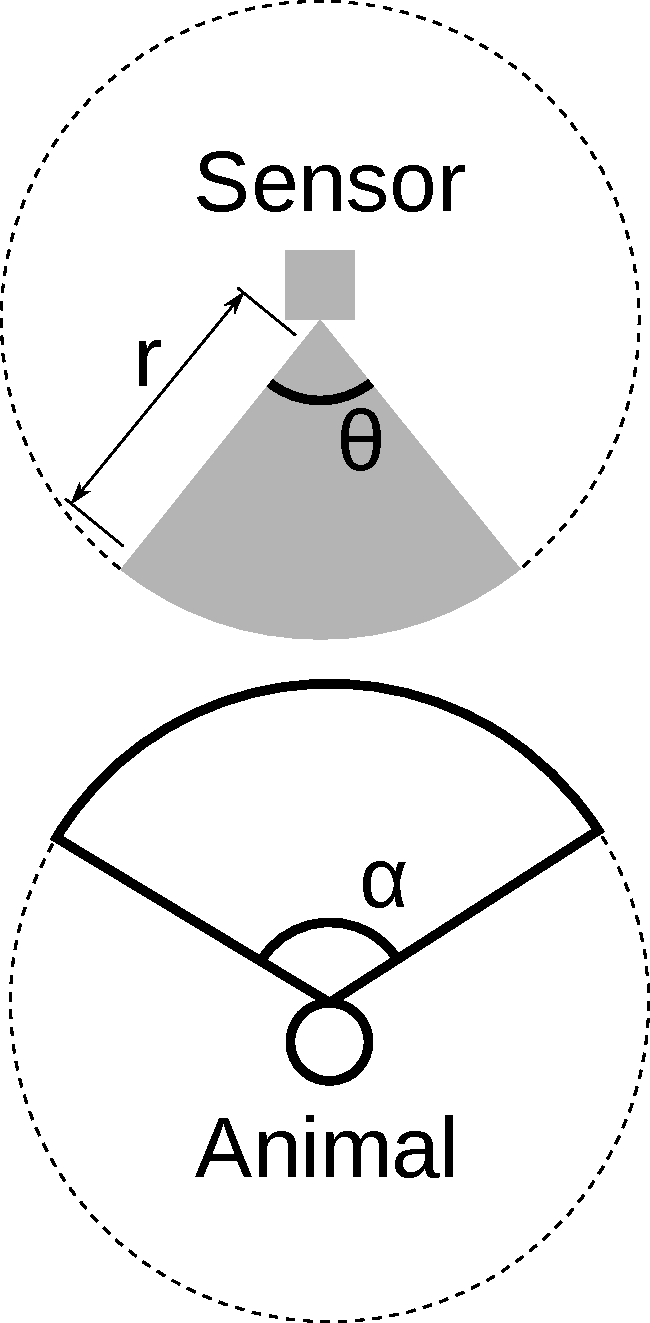
\includegraphics[width=4cm]{imgs/angleDefinitions.pdf}

\caption{Representation of sensor detection width and animal signal width. The filled square and circle represent a sensor and an animal, respectively; $\theta$, sensor detection width (radians); $r$, sensor detection distance; dark grey shaded area, sensor detection zone; $\alpha$, animal signal width (radians). Dashed lines around the filled square and circle represents the maximum extent of $\theta$ and $\alpha$, respectively.} % needs new description for the sensor detection zone  
\label{f:AngleDef}
\end{figure}



\subsubsection{Gas Model}

Following \cite{yapp1956theory}, we derive the gas model where sensors can capture animals in any direction and animal's signal is detectable from any direction($ \theta =  2\pi$ and $ \alpha =  2\pi$). We assume that animals are in a homogeneous environment, and move in straight lines of random direction with velocity $v$. We allow that our stationary sensor can capture animals at a detection distance $r$ and that if an animal moves within this detection zone they are captured with a probability of one, while animals outside the zone are never captured.

In order to derive animal density, we need to consider relative velocity from the reference frame of the animals. Conceptually, this requires us to imagine that all animals are stationary and randomly distributed in space, while the sensor moves with velocity $v$. If we calculate the area covered by the sensor during the survey period we can estimate the number of animals the sensor should capture. As a circle moving across a plane, the area covered by the sensor per unit time is $2rv$. The number of expected captures, $z$, for a survey period of $t$, with an animal density of $D$ is $z = 2rvtD$. To estimate the density, we rearrange to get $D = z/2rvt$.

\subsubsection{gREM derivations for different detection and signal widths}
Different combinations of $\theta$ and $\alpha$ would be expected to occur (e.g., sensors have different detection widths and animals have different signal widths). For different combinations $\theta$ and $\alpha$, the area covered per unit time is no longer given by $2rv$. Instead of the size of the sensor detection zone having a diameter of $2r$, the size changes with the approach angle between the sensor and the animal. For any given signal width and detector width and depending on the angle that the animal approaches the sensor, the width of the area within which an animal can be detected is called the profile, $p$. The size of the profile (averaged across all approach angles) is defined as the average profile $\bar{p}$. However, different combinations of $\theta$ and $\alpha$ need different equations to calcuate $\bar{p}$. 

\begin{figure}
\centering
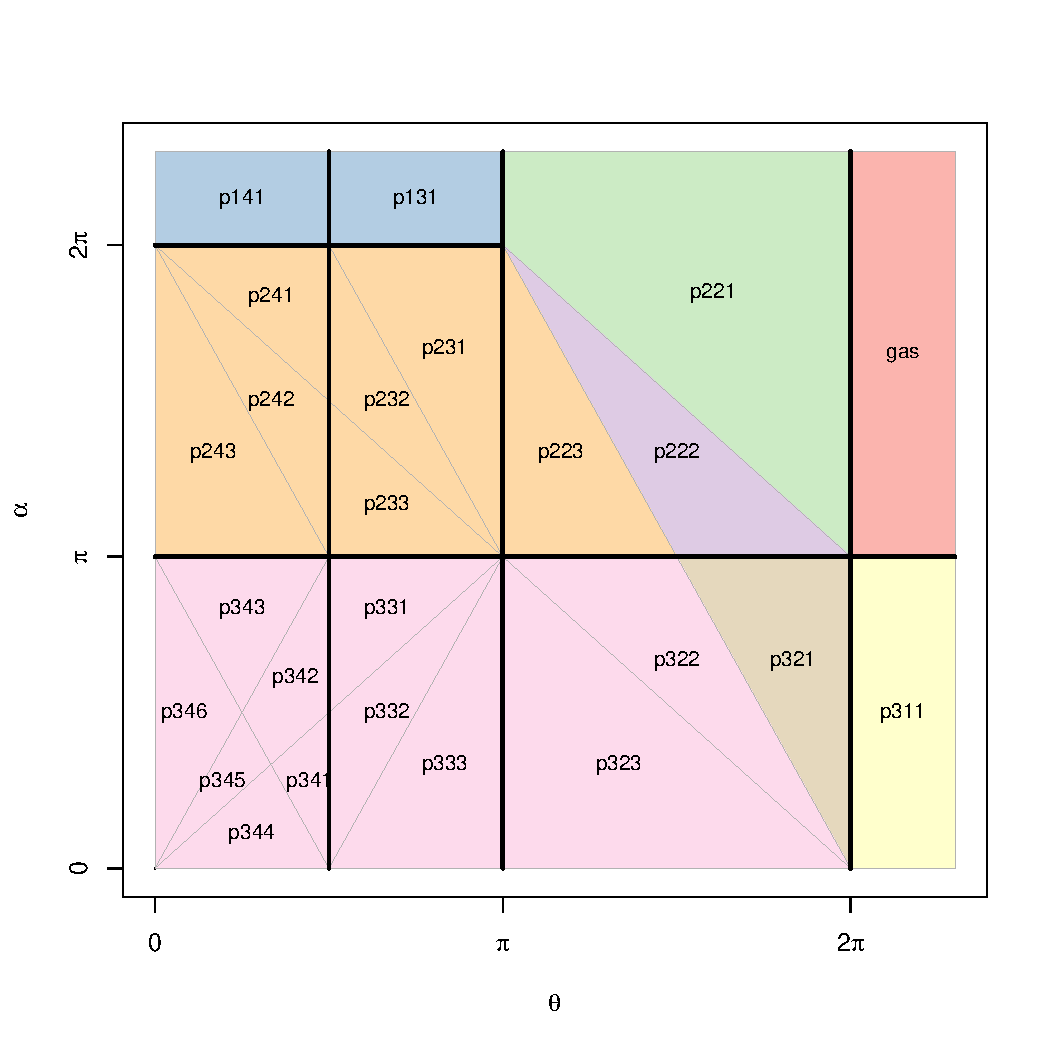
\includegraphics[width=7cm]{imgs/equalRegions.pdf}
\caption{Locations where derivation of the average profile $\bar{p}$ is the same for different combinations of sensor detection width and animal signal width. Symbols within each polygon refer to each gREM submodel named after their compass point, except for Gas and REM which highlight the position of these previously derived models within the gREM.}
\label{f:equalRegions}
\end{figure}

We have identified the parameter space for the combinations of $\theta$ and $\alpha$ for which the derivation of the equations are the same (defined as sub-models in the gREM) (Figure~\ref{f:equalRegions}). For example, the gas model becomes the simplest gREM sub-model (upper right in (Figure~\ref{f:equalRegions}) and the REM from \citep{rowcliffe2008estimating} is another gREM sub-model where $\theta<\pi/2$ and $\alpha = 2\pi$. We derive one gREM sub-model SE2 as an example below (where $4 \pi - 2 \alpha < \theta < 2\pi ,\; 0 < \alpha <\pi$) (see Appendix S2 for other gREM sub-models).

\subsubsection{Example derivation of SE2}

In order to calculate $\bar{p}$, we have to integrate over the focal angle, $x_1$ (Figure~\ref{f:xOne}). This is the angle taken from the centre line of the sensor. Other focal angles are possible ($x_2$, $x_3$, $x_4$) and are used in other gREM sub-models (see Appendix S2). As the size of the profile depends on the approach angle, we present the derivation across all approach angles. When the sensor is directly approaching the animal $x_1  = \pi/2$.

Starting from $x_1 = \pi/2$ until $\theta/2 + \pi/2 - \alpha/2$, the size of the profile is $2r\sin \alpha/2$ (Figure~\ref{f:firstInt}). During this first interval, the size of $\alpha$ limits the width of the profile. When the animal reaches $x_1$  = $\theta/2 + \pi/2 - \alpha/2$ (Figure~\ref{f:secondInt}), the size of the profile is $r\sin( \alpha/2) + r\cos( x_1  - \theta/2)$ and the size of $\theta/$ and $\alpha$ both limit the width of the profile (Figure~\ref{f:secondInt}). Finally, at $x_1  = 5\pi/2 - \theta/2  - \alpha/2$ until $x_1  = 3\pi/2$, the width of the profile is again $2r\sin\alpha/2$ (Figure~\ref{f:thirdInt}) and the size of $\alpha$ again limits the width of the profile. 

%insert new figure
\begin{figure}[t]
        \centering
	\begin{subfigure}[t]{60mm}
                \centering
		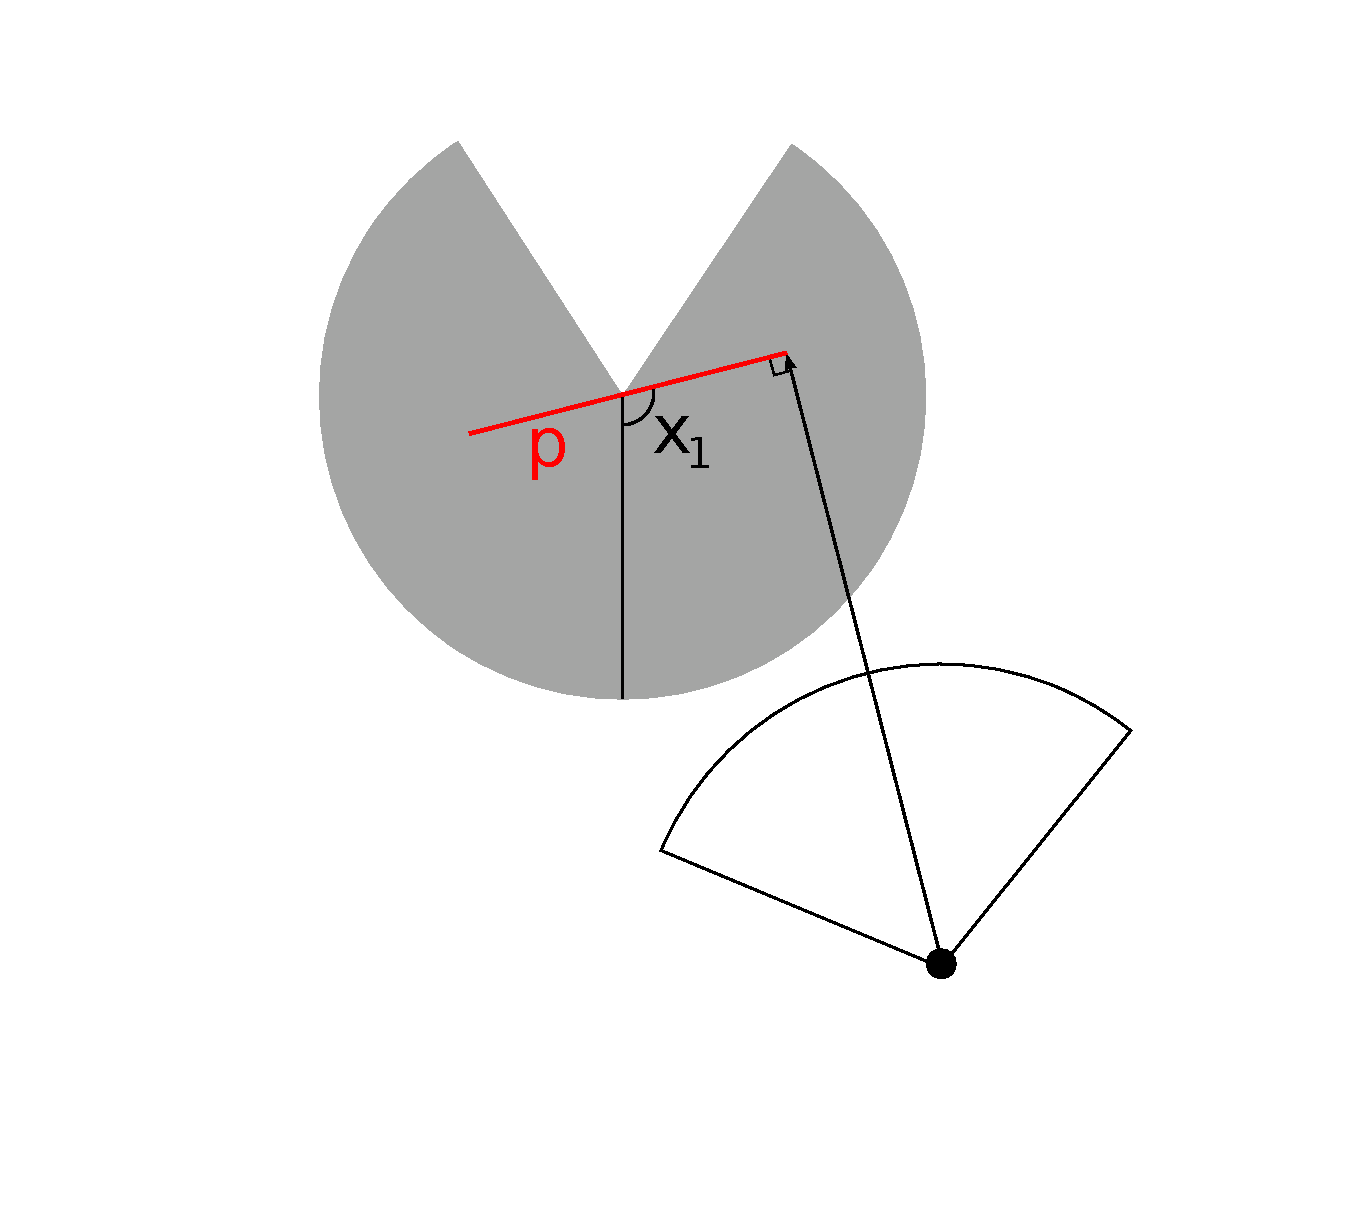
\includegraphics[width=60mm, trim= 6cm 2cm 6cm 0.3cm]{imgs/x1.pdf}
                \caption{}
                \label{f:xOne}
        \end{subfigure}%%
	~ 
	\begin{subfigure}[t]{60mm}
                \centering
		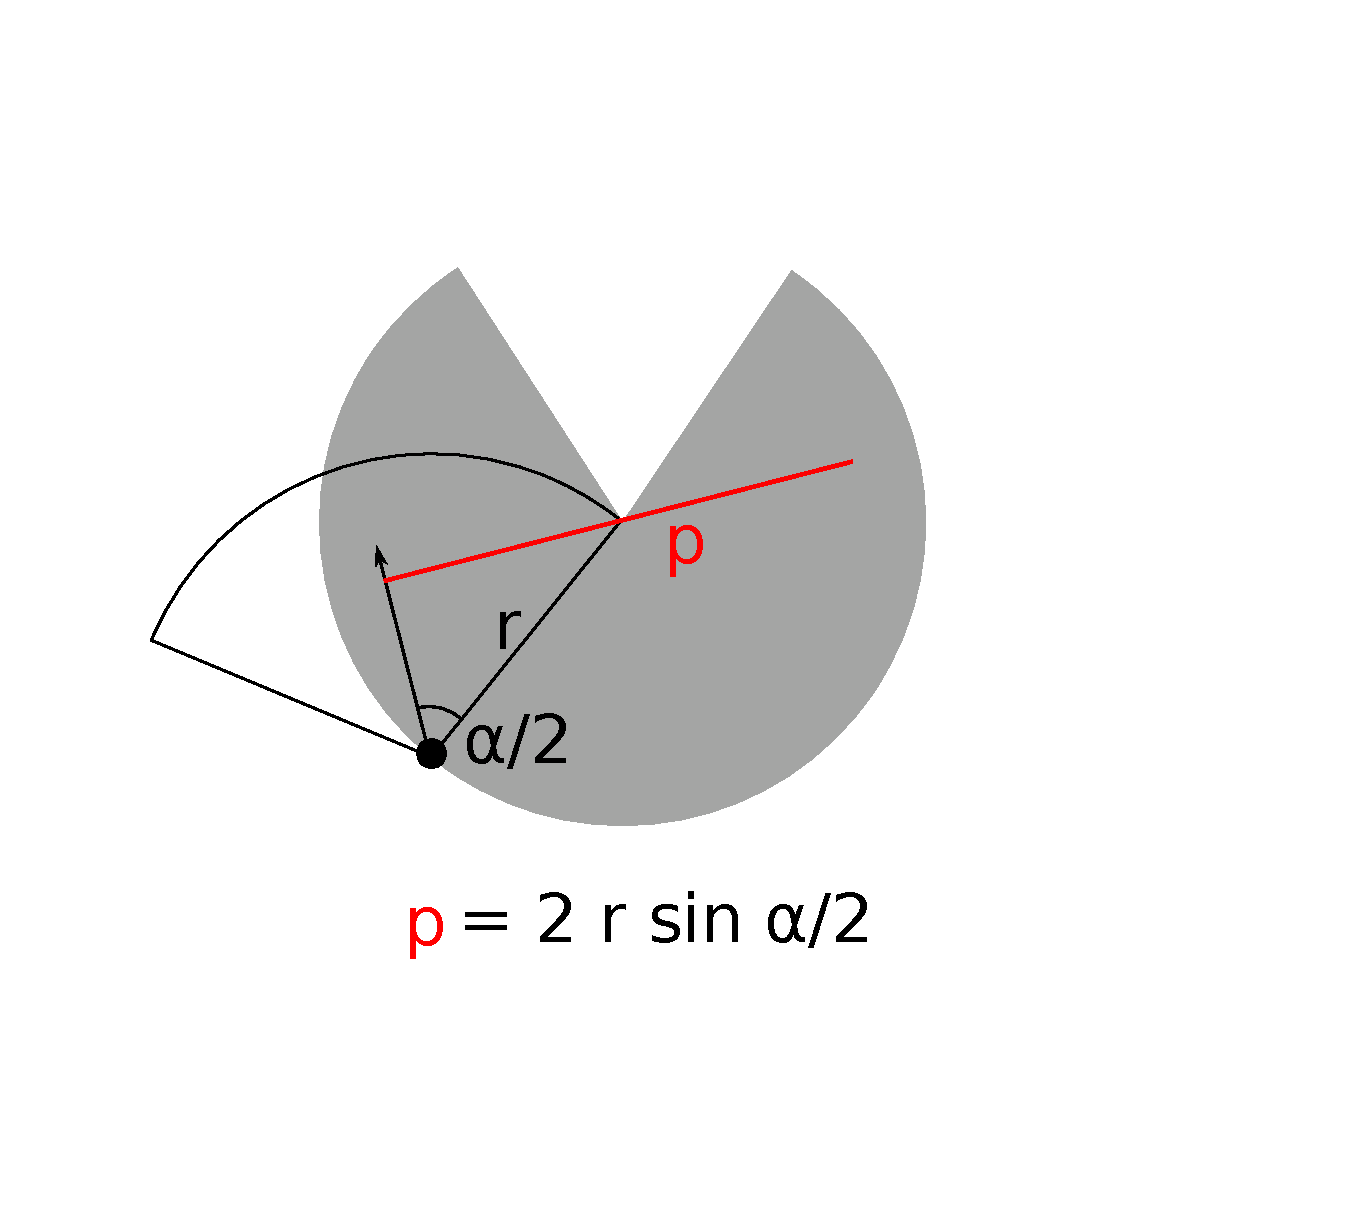
\includegraphics[width=60mm, trim= 6cm 2cm 6cm 4cm]{imgs/firstIntegral.pdf}
                \caption{}
                \label{f:firstInt}
        \end{subfigure}%%
	 
	\begin{subfigure}[t]{60mm}
                \centering
		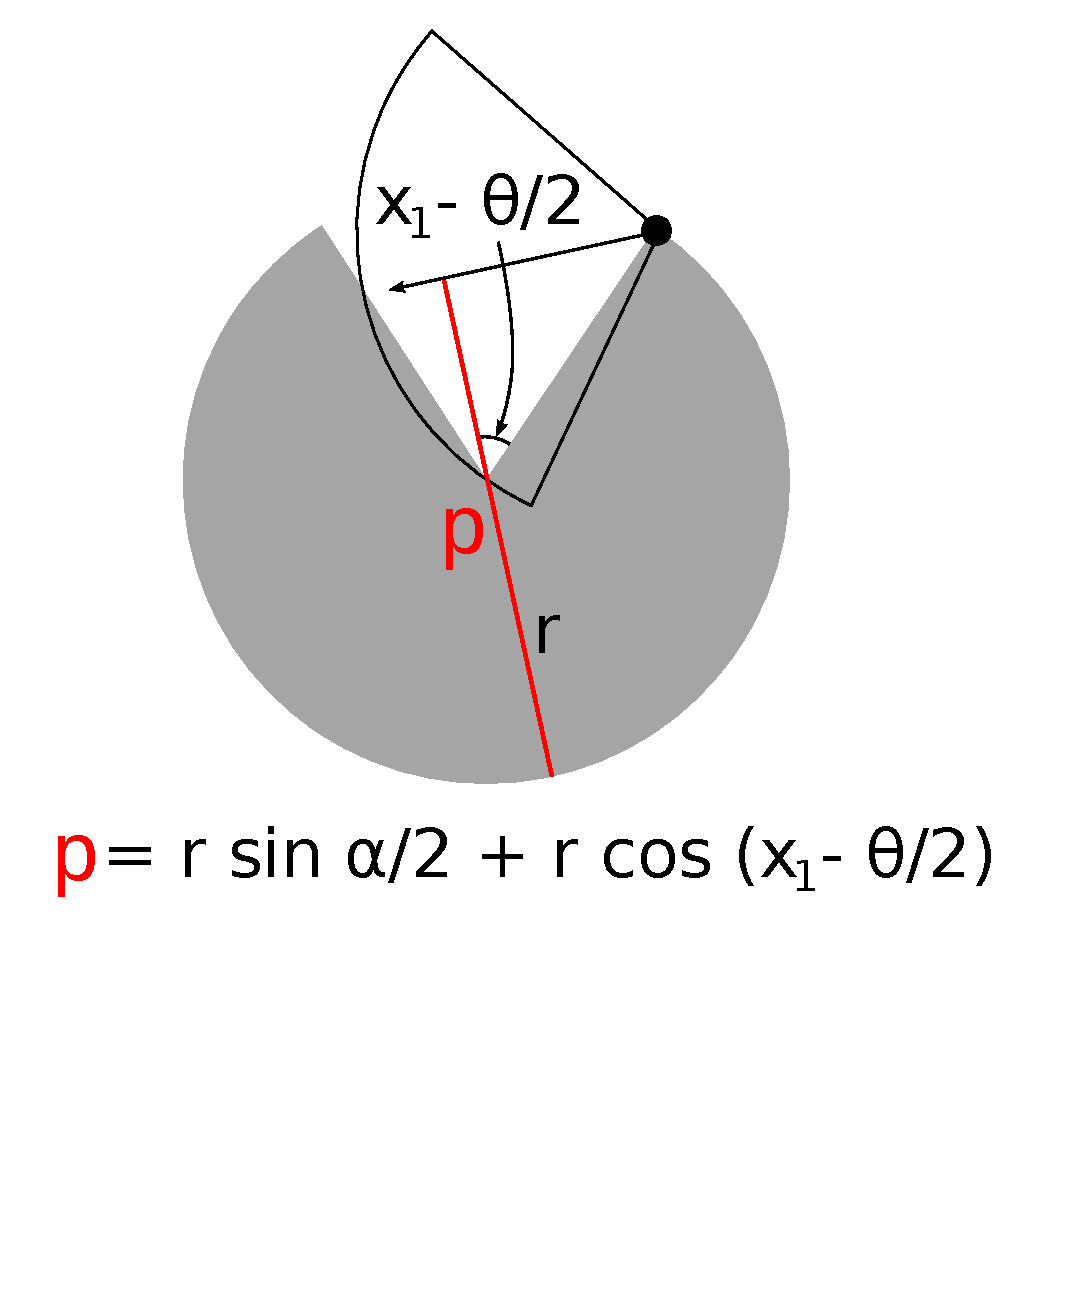
\includegraphics[width=60mm, trim= 6cm 2cm 6cm 1cm]{imgs/secondIntegral.pdf}
                \caption{}
                \label{f:secondInt}
        \end{subfigure}%%
	~ 
	\begin{subfigure}[t]{60mm}
                \centering
		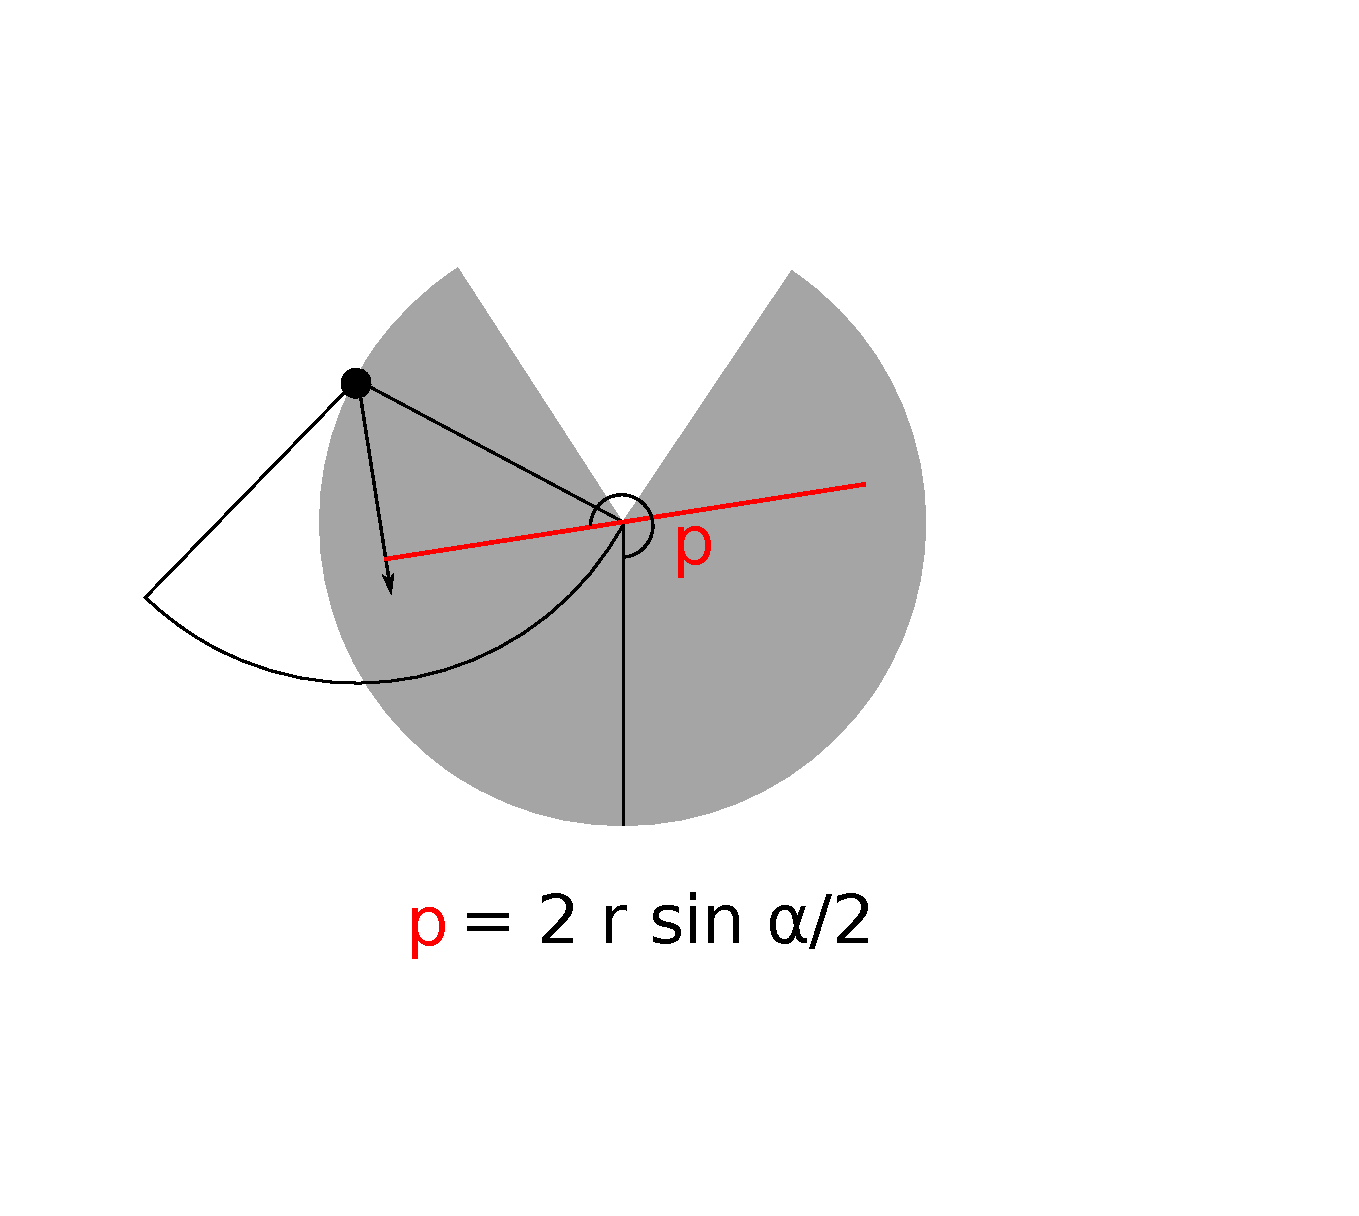
\includegraphics[width=60mm, trim= 6cm 2cm 6cm 4cm]{imgs/thirdIntegral.pdf}
                \caption{}
                \label{f:thirdInt}
        \end{subfigure}%%
\label{f:x1AndInt}
\caption{An overview of the derivation of SE2. The filled circles represent animals, with the animal signal shown as a unfilled sector and the direction of movement shown as an arrow. The detection zone of the sensors are shown as filled grey sectors with a detection distance of $r$. The SYMBOL shows the direction the sensor is facing;  $\theta$, sensor detection width; $\alpha$, animal signal width. The profile $p$ (the line an animal must pass through in order to be captured) is shown in red and $x_1$ is the focal angle, where (a) shows the location of $x_1$. The derivation of $p$ changes as the animal approaches the sensor from different directions where (b) is the derivation of $p$ when $x_1$ is in the interval $\lbrack\frac{\pi}{2}, \frac{\pi}{2} + \frac{\theta}{2} - \frac{\alpha}{2}\rbrack$, (c)  $p$ when $x_1$ is in the interval $\lbrack\frac{\pi}{2} + \frac{\theta}{2} - \frac{\alpha}{2}, \frac{5 \pi}{2} - \frac{\theta}{2} - \frac{\alpha}{2} \rbrack$ and (d) $p$ when $x_1$ is in the interval $\lbrack\frac{5 \pi}{2} - \frac{\theta}{2} - \frac{\alpha}{2}, \frac{3 \pi}{2}\rbrack$. The resultant equation for $p$ is shown beneath each figure.}
\end{figure}

The profile width $p$ for $\pi$ radians of rotation (from directly towards the sensor to directly behind the sensor) is completely characterised by the three intervals (Figure \ref{f:firstInt}--\ref{f:thirdInt}). Average profile width $\bar{p}$ is calculated by integrating these profiles over their appropriate intervals of $x_1$ and dividing by $\pi$ which gives

\begin{align}
    \bar{p} &=\frac{1}{\pi} \left(\int\limits_{\frac{\pi}{2}}^{\frac{\pi}{2} + \frac{\theta}{2} - \frac{\alpha}{2}}2 r \sin{\frac{\alpha}{2} }\;\mathrm{d}x_1+\int\limits_{\frac{\pi}{2} + \frac{\theta}{2} - \frac{\alpha}{2}}^{\frac{5 \pi}{2} - \frac{\theta}{2} - \frac{\alpha}{2}}r \sin{\frac{\alpha}{2} } + r \cos{\left (x_1 - \frac{\theta}{2} \right )}\;\mathrm{d}x_1+\int\limits_{\frac{5 \pi}{2} - \frac{\theta}{2} - \frac{\alpha}{2}}^{\frac{3 \pi}{2}}2 r \sin{\frac{\alpha}{2} }\;\mathrm{d}x_1\right) \nonumber  \\
     &= \frac{r}{\pi} \left(\theta \sin{\frac{\alpha}{2} } - \cos{\frac{\alpha}{2} } + \cos{\left (\frac{\alpha}{2} + \theta \right )}\right) \label{e:p321}
\end{align}

We then, as with the gas model, use this expression to calculate density
\begin{equation}
\label{e:gas}
D = z/vt\bar{p}
\end{equation}


%fix this @Tim
gREM submodels differ discontinuously (figure 2) at differnt combinations of alpha and theta because the number and nature of intervals needed to describe the average profile width changes.  
Examine the profile at $x_1 = 	\theta/2 + \pi/2$ (the profile is perpendicular to the edge of the blind spot.) We see that there is potentially a case where the left side of the profile is $r\sin \alpha/2$ while the right side is zero. This profile does not exist if we return to the full $2r\sin \alpha/2$ profile before $x_1  = \theta/2 + \pi/2$. Therefore we solve $5\pi/2 - \theta/2 - \alpha/2 <  \theta/2 + \pi/2$. We find that this new profile only exists if $ \alpha < 4\pi - 2 \theta$. This inequality defines the line separating models SE2 and its neighbouring model, SE3.

gREM submodel specifications were done by hand, and the integration was done using SymPy \citep{sympy} in Python (Appendix S3). The gREM submodels were checked by confirming that: 1) submodels adjacent in parameter space were equal at the boundary between them; 2) submodels that border $ \alpha = 0$ had$p = 0$ when $ \alpha = 0$; 3) average profile widths $\bar{p}$ were between 0 and $2r$ and; 4) each integral, divided by the range of angles that it was integrated over, was between 0 and $2r$. The scripts for these tests are included in Appendix S3 and the R \citep{R} implementation of the gREM is given in Appendix S4.  

\subsection{Simulation Model}

We tested the accuracy and precision of the gREM by developing a spatially explicit simulation of the interaction of sensors and animals using different combinations of sensor detection widths, animal signal widths, number of captures, and models of animal movement. 100 simulations were run where each consisted of a  \SI{7.5}{\kilo\meter} by \SI{7.5}{\kilo\meter} square (with periodic boundaries). A stationary sensor of radius $r$ was set up in the exact centre of each simulation, covering 7 sensor detection widths $\theta$ between 0 and $2\pi$( $2/9\pi$, $4/9\pi$, $6/9\pi$, $8/9\pi$, $10/9\pi$, $14/9\pi$, $2\pi$). Each simulation was populated with a density of \SI{70}{\animals\per\kilo\meter\squared}. This density was chosen as it is approximately the expected density of mammals animals weighing \SI{1}{\gram} calculated form the equation in \cite{damuth1981population}. This created a total of 3937 individuals per simulation which were placed randomly at the start of the simulation. Individuals were assigned x signal detection widths $\alpha$ between 0 and $\pi$ (x,x,x,x,x).

Each simulation lasted for $N$ steps (xx) of duration $T$ (15 minutes) giving a total duration of 150 days. The individuals moved within each step with a distance $d$, with an average speed, $v$. $d$, was sampled from a normal distribution with mean distance, $\mu_d = vT$, and standard deviation $\sigma_d = vT/10$. An average speed, $v = $ \SI{40}{\kilo\meter \per \day}, was chosen as this represents the largest day range of terrestrial animals \citep{carbone2005far}, and represents the upper limit of realistic speeds. At the end step, individuals were allowed to either remain stationary for a time step (with a given probability, $S$), change direction ($A$) between 0 and $\pi$. This resulted in 7 different movement models where: (1) simple movement, where $S$ and $A$ = 0; (2)stop-start movement, where (i) $S$ = 0.25, $A$ = 0, (ii) $S$ = 0.5, $A$ = 0, (iii) $S$ = 0.75, $A$ = 0; (3) random walk movement, where (i) $S$ = 0, $A$ = $\pi/3$, (ii) $S$ = 0, $A$ = $2\pi/3$, iii) $S$ = 0, $A$ = $\pi$.  
Individuals were counted as they moved in and out of the detection zone of the sensor per simulation. 

We calculated the estimated animal density from the gREM by summing the number of captures per simulation and inputting these values into the correct gREM submodel. gREM accuracy was determined by comparing the density in the simulation with the estimated density. High accuracy is indicated by the mean difference between the estimated and actual values converging to zero as sample size increases. gREM precision was determined by the standard deviation of estimated densities. We constructed box plots of the error between real and estimated densities to graphically test for accuracy and precision. 

We compared the accuracy and precision of all the gREM submodels. As these submodels are derived for different combinations of $\alpha$ and $\theta$, we used the gREM submodel accuracy and precision to determine the impact of different values of $\alpha$ and $\theta$. The impact of the number of captures and animal movement models on accuracy and precision was investigated using 4 different gREM submodels representative of the range $\alpha$ and $\theta$ values (submodels NW1, SW1, NE1, and SE3, Figure~\ref{f:equalRegions}). Using these four submodels, we calculated how long the simulation needed to run to generate a range of different capture numbers (from 10 to 100 captures in 10 unit intervals), and estimated animal density. These estimated densities were compared to the real density to assess the impact on the accuracy and precision on the gREM of different simulation lengths. We also used these four submodels to compare the accuracy and precision of a simple movement model, to stop-start movement models and random walk movement models. The gREM assumes that individuals move continuously with straight-line movement (simple movement model) and we therefore assess the impact of breaking the gREM assumptions. 


\section{Results}

\subsection{Analytical model}

Model results have been derived for each zone with all models except the gas model and REM being newly derived here. However, many models, although derived separately, have the same expression for $p$. Figure~\ref{f:equalModelResults} shows the expression for $p$ in each case. The general equation for density, using the correct expression for $p$ is then substituted into \ref{e:gas}.

Although more thorough checks are performed in Appendix S3, it can be seen that all adjacent expressions in Figure~\ref{f:equalModelResults} are equal when expressions for the boundaries between them are substituted in.

\begin{figure}
	\centering
	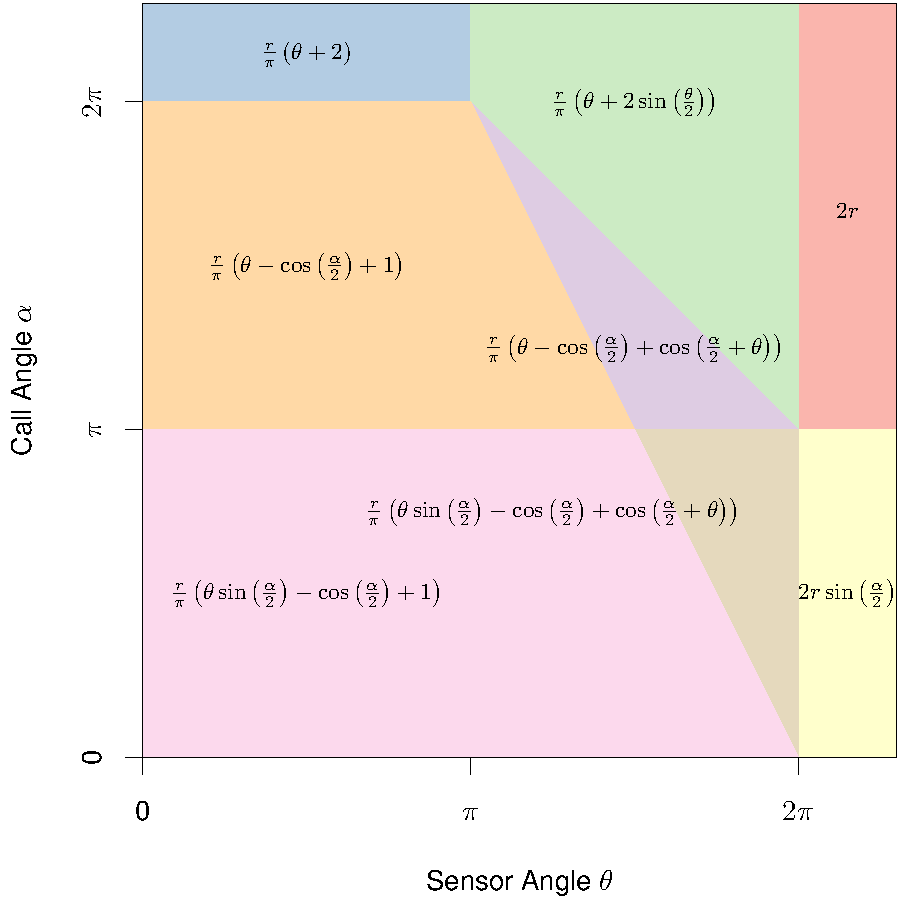
\includegraphics[width=7cm]{imgs/equalModelResults.pdf}
	\caption{Equations for the profile wide, $p$, given sensor and call widths. Each colour block represents one equation, despite independent derivation within each block, many models result in the same expression. These are collected together and presented as one block of colour.}
	\label{f:equalModelResults}
\end{figure}



\subsection{Simulation model}

\begin{figure}
	\centering
	\begin{subfigure}[t]{60mm}
		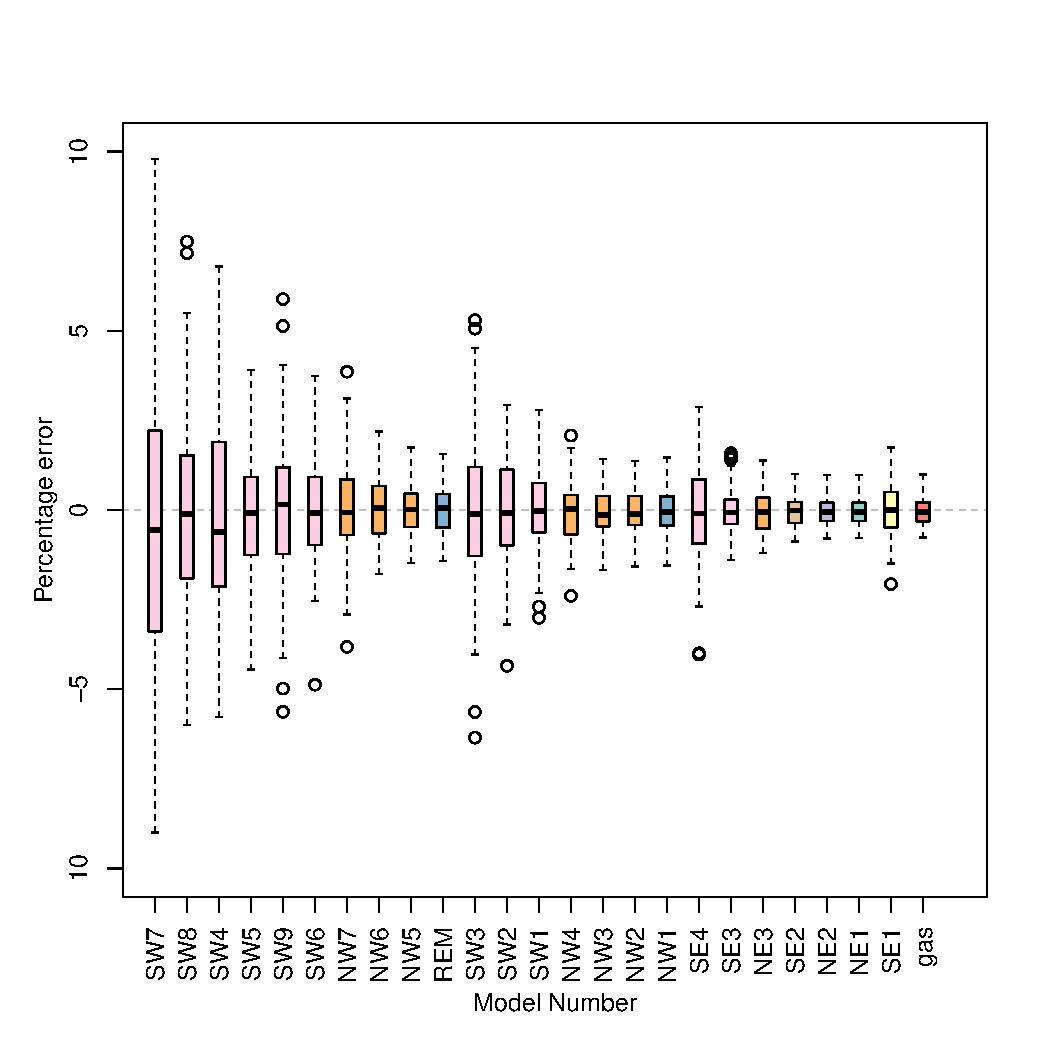
\includegraphics[width=60mm]{imgs/AverageModelBias.pdf}
		\label{f:ModelBias}
		\caption{} 
	\end{subfigure}
	~
	\begin{subfigure}[t]{60mm}
		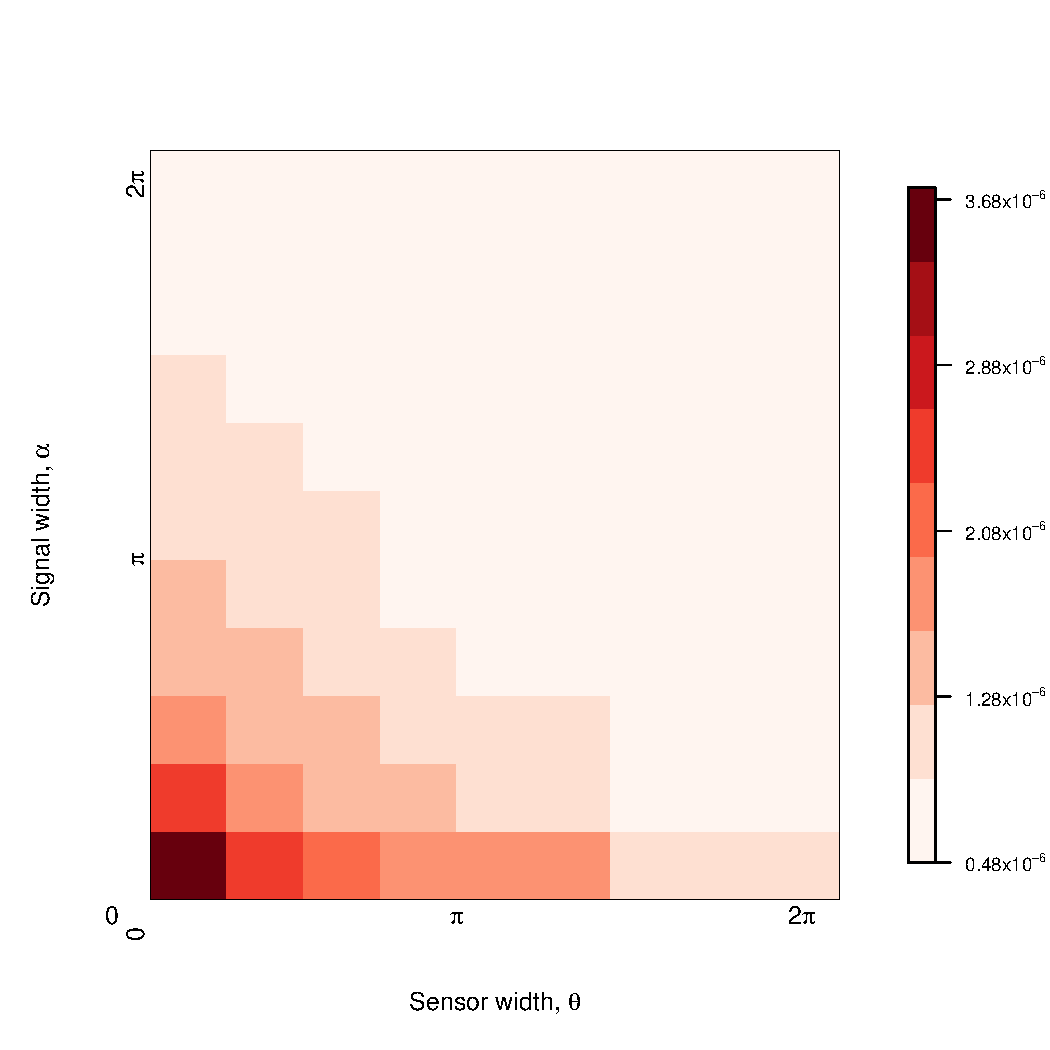
\includegraphics[width=60mm]{imgs/ResultStandardDeviation.pdf}
		\label{f:StandardDevaition}
		\caption{} 
        \end{subfigure}
        \caption{The precision of the gREM given a range of detection and call angles. The standard deviation of the percentage error for sensor, and call angles between 0 and $2\pi$ where: $r = $ \SI{100}{\meter}; $T = $ \SI{150}{\day}; $v = $ \SI{40}{\kilo\meter\per\day}; $D = $ \SI{70}{\animals\per\kilo\meter\squared}; and with detection angles varying between models. Where red indicates a high standard deviation and blue represents a low standard deviation.} 
	\label{f:AccAndPrec}
\end{figure}

For each model we compared the estimated densities to the true densities in a simulation. None of the models showed any evidence of any significant differences between the estimated and true density values (Figure~\ref{f:ModelBias}). The precision of the models do vary however. The standard deviation of the error is strongly related to the call and sensor width (Figure~\ref{f:StandardDevaition}), such that larger widths have greater precision. However, even the models with small call and sensor angles have a relativity high level of precision. 

\begin{figure}[t]
       \centering
	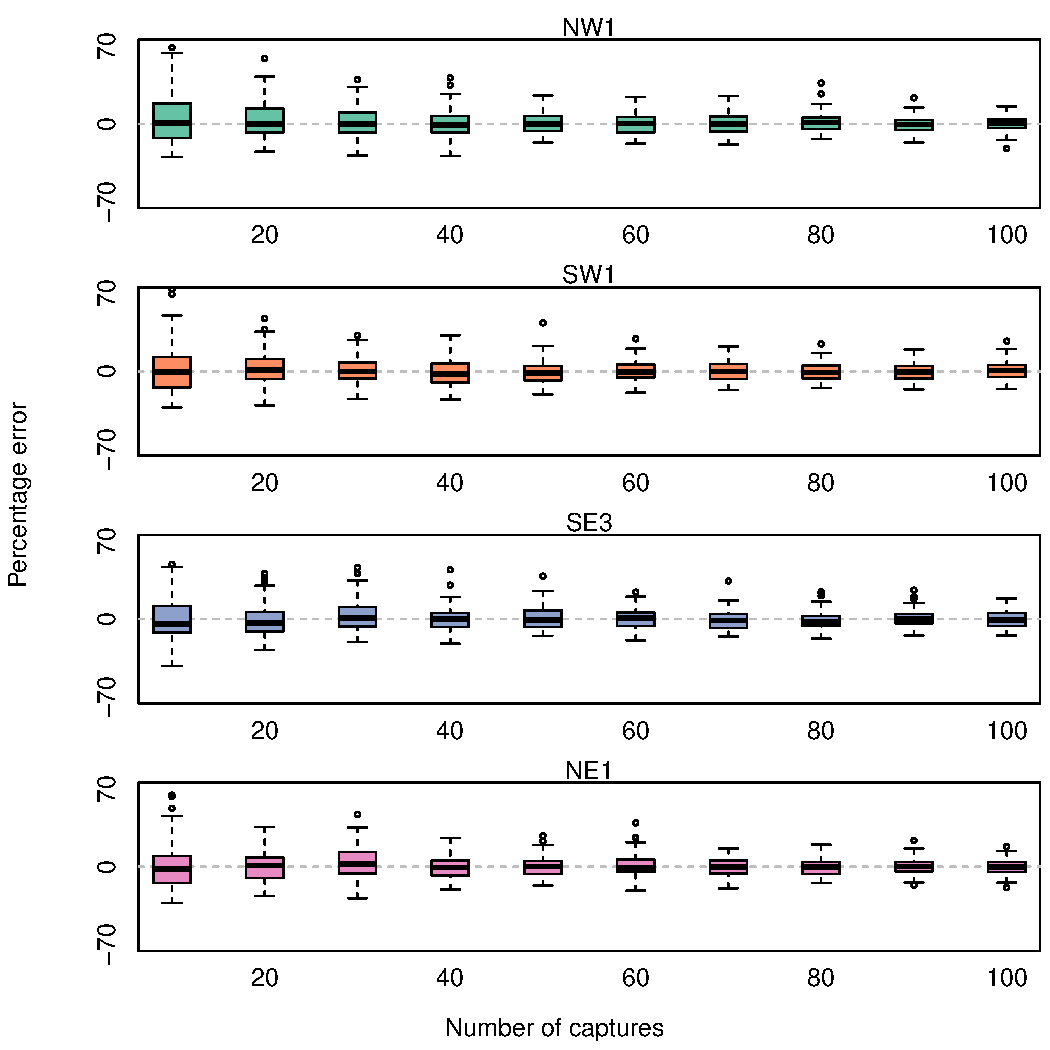
\includegraphics[width=7cm]{imgs/ResultsNoCaptures.pdf}
           \label{f:Captures}
        \caption{Accuracy of the gREM reminds unchanged, whilst precision increases, with captures. Boxplots of four test models when given different numbers of captures where: $r = $ \SI{100}{\meter}; $T = $ \SI{150}{\day}; $v = $ \SI{40}{\kilo\meter\per\day}; $D = $ \SI{70}{\animals\per\kilo\meter\squared}; and with angles varying between models. Where the model names refer to Figure 1 in Appendix S2.} 
\end{figure}

The precision of the model is dependent on the number of captures during the survey. In Figure~\ref{f:Captures} we can see that the model precision gets greater as the number of captures increase. As the number of captures reaches about 100 then the coefficient of variation falls below 10\% which could be considered negligible. %The number of captures is highly dependent on the speed of the animals, the size of the detection zone, and the length of the survey, as these values increase the number of captures is also likely to increase. 

\subsubsection{Use of the gREM when animal movement is not consistent with model assumptions}

 Simulating start-stop instead of continuous movement had no effect the accuracy, or the precision, of the estimates (Figure~\ref{f:Perch}) as long as the true overall speed of the animal is known. Relaxing straight line movement to allow random or correlated random walks did not effect the accuracy of the method (Figure~\ref{f:Tort}). We allowed animals to change direction up to a maximum value at the end of each step, picked from a uniform distribution where the maximum angle ranged from 0 to $\pi$, which corresponds to straight line movement and random walk respectively. There is no significant difference in the variance for the change, this could be because of the between the step length of the animal movement, 15 minutes, means that immediate double counting of the same animal is unlikely.  In the case where large directional changes are likely to occur within short periods of time leading to double counting of the same animal within a short period of time may need to be adjusted because of this. 

\begin{figure}[t]
	\centering
	\begin{subfigure}[t]{60mm}
      		\centering
		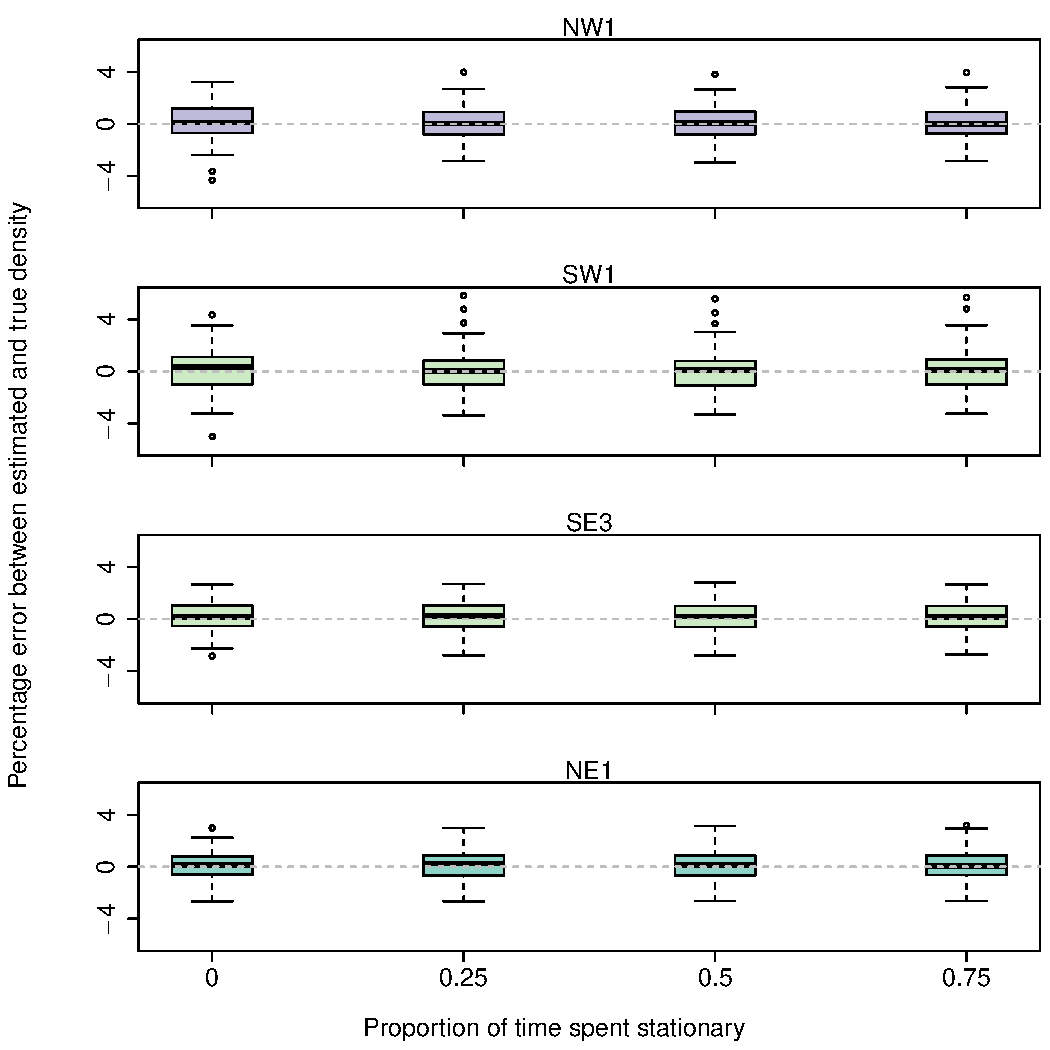
\includegraphics[width=60mm]{imgs/ResultsPerch.pdf}
         	 \label{f:Perch}
		\caption{} 
	\end{subfigure}
	~
	\begin{subfigure}[t]{60mm}
                \centering
		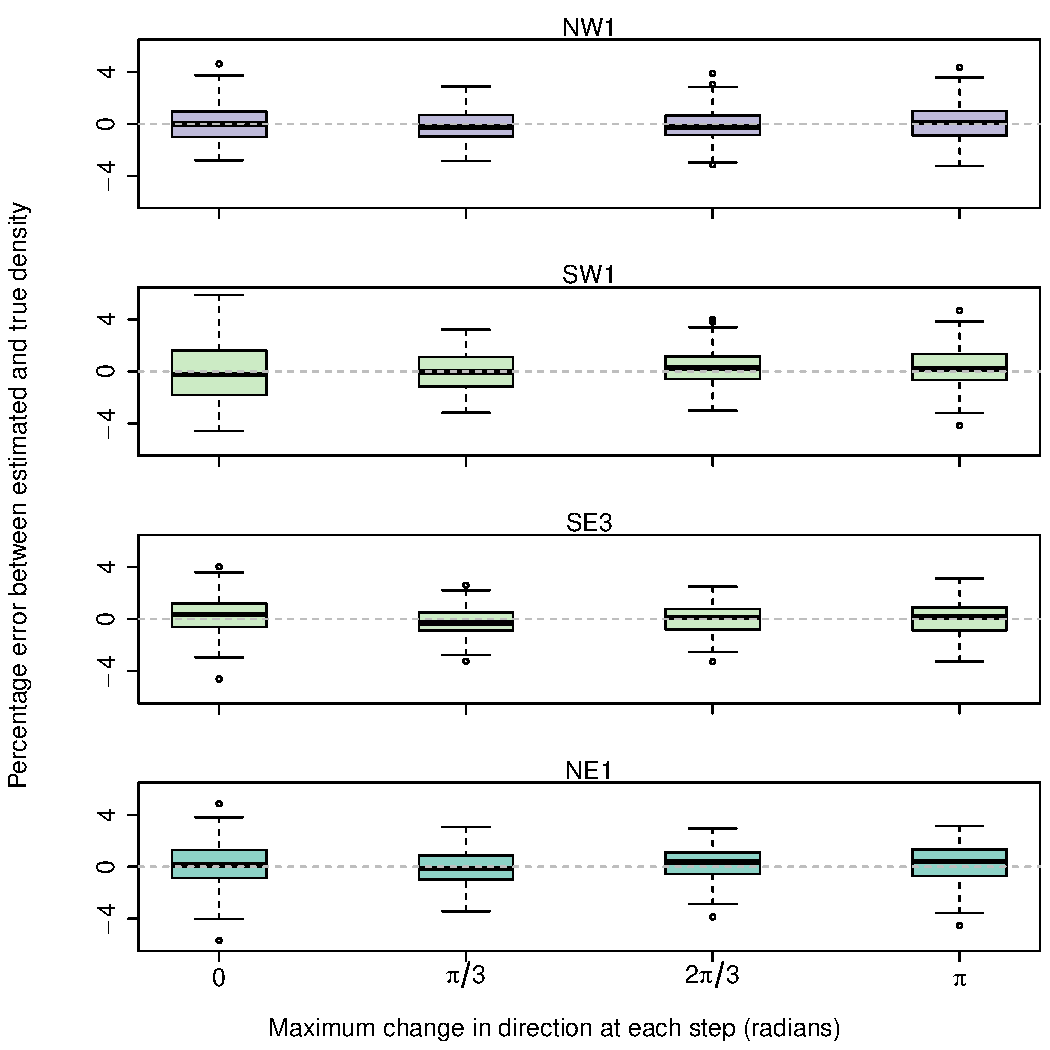
\includegraphics[width=60mm]{imgs/ResultsTort.pdf}
                \label{f:Tort}
                \caption{} 
         \end{subfigure}
	\label{f:BreakAssump}
	\caption{
	%perch
	Accuracy and the precision of the gREM given changes in the amount of time an animal spends stationary on average. Distribution of model error when simulated animals spend increasing proportion of time stationary where:  $r = $ \SI{100}{\meter}; $T = $ \SI{150}{\day}; $v = $ \SI{40}{\kilo\meter\per\day}; $D = $ \SI{70}{\animals\per\kilo\meter\squared}; and with detection angles varying between models. Where the model names refer to Figure 1 in Appendix S2. 
	%Tort
	Accuracy and the precision of the gREM given different types of correlated walks. Distribution of model error when simulated animals move with different types of correlated walk where:  $r = $ \SI{10}{\meter}; $T = $ \SI{352}{\day}; $v = $ \SI{40}{\kilo\meter\per\day}; $D = $ \SI{70}{\animals\per\kilo\meter\squared}; and with angles varying between models. Where the model names refer to Figure 1 in Appendix S2.} 
\end{figure}

                  
                  
%%%% ------- Discussion ---------%%%%
\section{Discussion}


We have developed the gREM such that it can be used to estimate density from acoustic and optical sensors. This has entailed a generalisation of the gas model and the model in \citep{rowcliffe2008estimating} to be applicable to any combination of sensor width and call directionality. We have used simulations to show, as a proof of principle, that these models are accurate and precise.

The gREM is therefore available for the estimation of density of a number of taxa of importance to conservation, zoonotic diseases and ecosystem services. The models provided are suitable for certain groups for which there are currently no, or few, effective methods for density estimation. Any species that would be consistently recorded at least once when within range of a detector would be a suitable subject for the gREM, such as bats \citep{kunz2009methods}, songbirds \citep{buckland2006point}, Cetaceans \citep{marques2009estimating} or forest primates \citep{hassel2008reliable}. Within increasing technological capabilities, this list of species is likely to increase dramatically.

Importantly the methods are noninvasive and do not require human marking or naturally identifying marks (as required for mark-recapture models). This makes them suitable for large, continuous monitoring projects with limited human resources. It also makes them suitable for species that are under pressure, species that cannot naturally be individually recognised or species that are difficult or dangerous to catch.

From our simulations  we believe that this method has the potential produce accurate and precise estimates for many different species, using either camera or acoustic detectors. When choosing detectors a researcher should pick the detector with the largest radius and detection angle possible, but whilst a small capture area may reduce precision there is only a limited impact on the overall precision of the model (Figure~\ref{f:StandardDevaition}). A range of factors will affect the overall precision of the model, like size of detection zone, speed of animal, density of animals and length of survey which are reflected in the number of captures. Increasing the number of captures leads to more precise estimates, for species which more slower, or have occur at lower densities, then the detection zone and length of survey need to be increased to compensate so that at least 100 captures are collected (Figure~\ref{f:Captures}).

Within the simulation we have assumed an equal density across the entire world, however in a field environment the situation would be much more complex, with additional variation coming from local changes in density between camera sites. We also assume perfect knowledge of the average speed of an animal and size of the detection zone, and instant triggering of the camera. All of which may lead to possible bias or decreased precision.    

Although we have used simulations to validate these models, much more robust testing is needed. Although difficult, proper field test validation would be required before the models could be fully trusted. Note, however, that the REM \citep{rowcliffe2008estimating} has been field tested. Both \citet{rowcliffe2008estimating} and \citet{zero2013monitoring} both found that the REM were effective manner of estimating animal densities \citep{rowcliffe2008estimating, zero2013monitoring}. There was some discrepancies between the REM and the census methodologies found by Rovero and Marshall which may have been down to lack of knowledge of wild animal speed, and an underestimate in census results \citep{rovero2009camera}. In some taxa gold standard methods of estimating animal density exist, such as capture mark recapture. Where these gold standard exist, and have been proved to work, a simultaneous gREM study could be completed to test the accuracy under field conditions. An easier way to continue to evaluate the models is to run more extensive simulations which break the assumptions of the analytical models. The main element that cannot be analytically treated is the complex movement of real animals. Therefore testing these methods against true animal traces, or more complex movement models would be useful.


There are a number of positive extensions to the gREM which could be developed in the future. The original gas model was formulated for the case where both subjects, either animal and detector, or animal and animal, are moving \citep{Hutchinson_Waser_2007}. Indeed any of the models with animals that are equally detectable in all directions ($\alpha = 2\pi$) can be trivially expanded for moving by substituting the sum of the average animal velocity and the sensor velocity for $v$ as used here. However, when the animal has a directional call, the extension becomes much less simple. The approach would be to calculate again the mean profile width. However, for each angle of approach, one would have to average the profile width for an animal facing in any direction (i.e. not necessarily moving towards the sensor) weighted by the relative velocity of that direction. There are a number of situations where a moving detector and animal could occur and as such may be advantage to have a method of estimating densities from the data collected, e.g. an acoustic detector based off a boat when studying Cetacea or sea birds \citep{yack2013passive}.

Another interesting, and so far unstudied problem, is edge effects caused by trigger delays (the delay between sensing an animal and attempting to record the encounter) and time expansion acoustic detectors which repeatedly turn on an off during sampling. Both of these have potential biases as animals can move through the detection zone without being detected. The models herein are formulated assuming constant surveillance and so the error quickly becomes negligible. For example, if it takes longer for the recording device to be switched on than the length of some animal calls there could be a systematic underestimation of density. 

%%%% ------- Acknowledgments ---------%%%%
\section{Acknowledgments}



\bibliographystyle{mee.bst}	
\bibliography{lucas-moorcroft-etal-refs.bib}	

\end{document}
>>>>>>> 3227269a1020a4e84e4420fda6931dc5b1d949b2
